%%
%% LaTeX Document Template
%%
\documentclass[sigplan,screen]{acmart}
%%
%% \BibTeX command to typeset BibTeX logo in the docs
\AtBeginDocument{%
  \providecommand\BibTeX{{%
    Bib\TeX}}}

%% Publication information - modify as needed
\setcopyright{acmlicensed}
\copyrightyear{2024}
\acmYear{2024}
\acmDOI{XXXXXXX.XXXXXXX}
\acmConference[]{University of Auckland}{University of Auckland}{2025}
\acmISBN{978-1-4503-XXXX-X/2024/XX}

%% Citation style configuration
%%\citestyle{acmauthoryear}


%%
%% end of the preamble, start of the body of the document source.
% Improve line breaking to avoid overfull boxes for long words
\emergencystretch=3em
\begin{document}

%%
%% The "title" command has an optional parameter,
%% allowing the author to define a "short title" to be used in page headers.
\title[Data Mining]{ A Fraud Detection Solution for Extremely Imbalanced Financial Data}

%% Author information
\author{Xiaoqing Miao}
\email{xmia665@aucklanduni.ac.nz}
\affiliation{%
  \institution{University of Auckland }
  \city{Auckland}
  \country{New Zealand}
}


%% Short author list for page headers
\renewcommand{\shortauthors}{Xiaoqing Miao}

%%
%% The abstract is a short summary of the work to be presented in the
%% article.
\begin{abstract}
\sloppy
Financial fraud detection faces significant challenges due to extreme class imbalance in transaction data. This study presents a comprehensive solution using the CRISP-DM methodology~\cite{shearer2000crisp} to transform a severely imbalanced dataset into an effective fraud detection system. Working with the PaySim synthetic dataset containing 6.36 million mobile payment transactions, where fraudulent cases represent only 0.13\% of all records, I developed a robust binary classification model achieving remarkable performance improvements. Through systematic data exploration, I identified that fraud occurs exclusively in CASH\_OUT and TRANSFER transactions. By implementing strategic undersampling to create a balanced training set, combined with careful feature engineering and selection, I built a logistic regression model that achieved 91.40\% accuracy, 0.976 AUC, 93.26\% precision, and 89.51\% recall on test data (on a class-balanced test set). The dramatic improvement from detecting 0.13\% fraud in raw data to achieving 91.40\% classification accuracy demonstrates the effectiveness of proper data mining techniques. This project not only surpassed all predefined success criteria (recall ≥85\%, precision ≥70\%, AUC ≥0.95) but also provides a reproducible framework for addressing class imbalance in fraud detection systems. The findings offer valuable insights for financial institutions seeking to enhance their fraud prevention capabilities while maintaining operational efficiency.
\fussy
\end{abstract}

%% CCS concepts and keywords - add your own
%% Generate CCS concepts at: https://dl.acm.org/ccs/ccs.cfm
%%\begin{CCSXML}
%%...your CCS XML here...
%%\end{CCSXML}
%%\ccsdesc[500]{Your primary concept}
%%\ccsdesc[300]{Your secondary concept}

%% Keywords
\keywords{fraud detection, class imbalance, CRISP-DM, logistic regression, PaySim dataset}

%% Optional teaser figure
%%\begin{teaserfigure}
%%  \includegraphics[width=\textwidth]{your-image}
%%  \caption{Your teaser figure caption.}
%%  \Description{Description of your teaser figure.}
%%  \label{fig:teaser}
%%\end{teaserfigure}

%% Submission dates (optional)
%%\received{Date}
%%\received[revised]{Date}
%%\received[accepted]{Date}

%%
%% This command processes the author and affiliation and title
%% information and builds the first part of the formatted document.
\maketitle

\section{Business/Situation Understanding}
\subsection{Business/Situation Objectives}
\textbf{Business Background}

The digital payment industry faces significant fraud challenges. The PaySim dataset simulates one month of mobile payment transactions, containing 6.3 million records, of which only 0.13\% (8,213 transactions) are fraudulent, reflecting the imbalanced conditions of the real world.
\textbf{Main Business Objectives}

\begin{itemize}
\item \textbf{Minimize financial loss:} Reduce fraud-related losses by 75\% through early detection.
\item \textbf{Protect customer trust:} Prevent customers from becoming fraud victims and maintain a customer satisfaction rate of over 90\%.
\item \textbf{Optimize operational efficiency:} Reduce the manual fraud investigation workload by 60\%.
\end{itemize}

\textbf{Business Success Criteria}

\begin{itemize}
\item \textbf{Detection performance:} Recall $\geq$ 85\%, Precision $\geq$ 70\%, AUC score $\geq$ 0.95.
\item \textbf{Operational efficiency:} Transaction processing time < 100 milliseconds, system availability $\geq$ 99.9\%.
\item \textbf{Financial impact:} A 10:1 return on investment (for every 1 USD invested, 10 USD in fraud losses can be prevented).
\end{itemize}

\textbf{Alignment with Data Mining Objectives}

The business objectives directly translate into:

\sloppy
\begin{itemize}
\item Building a binary classifier for fraud detection (fraud vs. legitimate).
\item Identifying high-risk patterns in TRANSFER and CASH\_OUT transactions.
\item Developing a real-time risk score for transaction approval decisions.
\end{itemize}
\fussy

Expected value: annual savings of USD 300,000--750,000 from fraud prevention, a USD 75,000 reduction in investigation costs, and an enhanced competitive position as a secure payment platform.

\subsection{ Assessment of the Situation}
\subsubsection{Resource Inventory}

As an individual student project, the available resources include: the PaySim open-source dataset (6.36 million transaction records), a personal laptop (8GB RAM), IBM SPSS Modeler Student Edition (licensed free through the university), and 2 weeks of project time. Knowledge resources include course materials, Kaggle dataset documentation, online tutorials, and relevant academic papers. As a student of the data mining course, I possess basic knowledge of classification algorithms and operational experience with SPSS Modeler.

\subsubsection{Requirements and Assumptions}

Requirements: Complete all phases of CRISP-DM, build a binary classification model capable of detecting fraudulent transactions, achieve a performance target of AUC > 0.9, and submit a comprehensive project report.

Assumptions: The PaySim synthetic data is assumed to represent real-world fraud characteristics; the laptop can handle 6 million records; 2 weeks is sufficient to complete all iterations; the SPSS Modeler Student Edition provides adequate functionality to support the project requirements.



\subsubsection{Constraints}

\begin{itemize}
\item \textbf{Time Constraint}: The project must be submitted within 2 weeks, with 15---20 hours available per week.
\item \textbf{Technical Constraint}: Limited by personal computer performance, data sampling may be required; the SPSS Student Edition may have functionality restrictions.
\item \textbf{Data Constraint}: Only public datasets can be used; real-world business data for validation is unavailable.
\item \textbf{Experience Constraint}: As a student, there is limited practical experience in financial fraud detection.
\end{itemize}



\subsubsection{Risks and Contingencies}

The project risk assessment identified five major risk areas, covering technology, performance, time, software, and data. Specific contingency plans were developed for each risk to ensure that the project can be completed successfully under unfavorable conditions, thereby maximizing the likelihood of achieving the project objectives.

\vspace{0.3cm}

\begin{center}
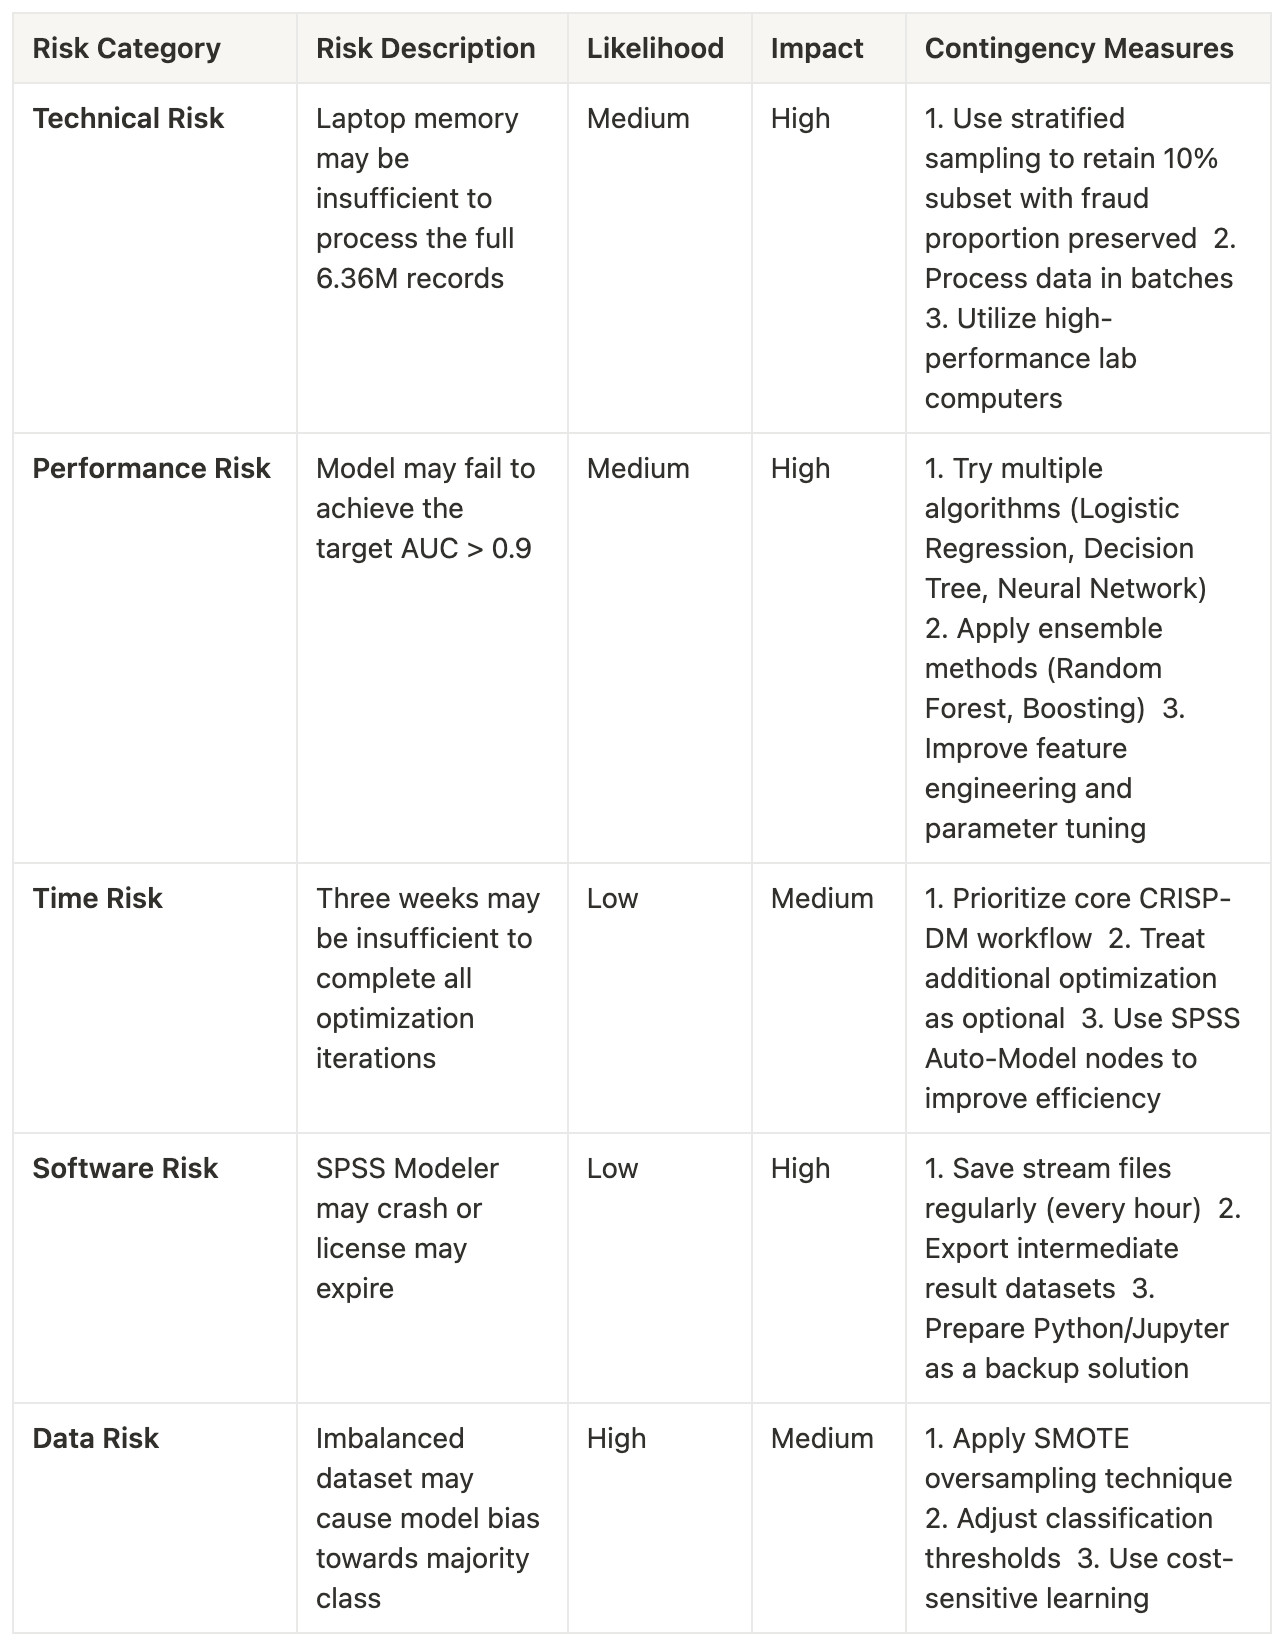
\includegraphics[width=0.9\columnwidth]{table1.jpg}
\vspace{0.2cm}

Table 1: Risk Assessment and Contingency Plans
\end{center}

\vspace{0.3cm}



\subsection{Data Mining Objectives}
    
    The primary objective of this project is to build an effective classification model to accurately predict the isFraud label in financial transactions. Specifically, the goal is to analyze various transaction features (e.g., type, amount, changes in account balances) to distinguish whether a transaction is normal (isFraud = 0) or fraudulent (isFraud = 1).
    
    \subsubsection{Model Evaluation Method}
    
    Given that fraudulent samples are far fewer than normal ones, the dataset suffers from severe class imbalance. Therefore, the traditional Accuracy metric can be misleading and will not be used as the main evaluation criterion.

Instead, this study adopts the ROC curve (Receiver Operating Characteristic Curve) and its Area Under the Curve (AUC) as the core evaluation metrics\cite{fawcett2006roc}. AUC measures the models'  overall ability to distinguish positive from negative samples, is insensitive to class imbalance, and is widely recognized as a reliable standard for this type of problem.    
    
\subsubsection{Success Benchmarks}
    
    To avoid setting business-detached rigid goals, I adopt a validity threshold + post hoc evaluation approach:

\begin{itemize}
\item \textbf{Validity Threshold (Necessary Condition):} The model's AUC on the testing set must be \textbf{significantly higher than 0.5} (e.g., lower bound of the 95\% CI of AUC > 0.5, or $p$ < 0.05 in DeLong's test against 0.5\cite{delong1988comparing}). If this is not satisfied, the model is considered \textbf{invalid}.
\item \textbf{Relative Evaluation (Performance Ranking):} Once the threshold is met, no fixed benchmark is pre-set. Instead, the model will be qualitatively assessed based on AUC, PR-AP, and confusion-matrix-derived metrics (Precision / Recall / F1). The results will then be rated qualitatively (e.g., ``Pass / Good / Excellent'') and discussed alongside the business trade-off between false positives and false negatives.
\end{itemize}
    
      Note: Significantly higher than 0.5 serves as the minimum validity criterion.
    
\subsubsection{ Model Interpretation and Deployment}
    
    The scope of this analysis is strictly limited to data preprocessing, model construction, and AUC-based performance evaluation. Deeper business interpretation of model results (e.g., feature importance analysis) and practical deployment strategies are beyond the scope of this project and will be considered as possible directions for future research.
\subsection{Project Plan}
The project plan outlines the major tasks of this study. I provide a Work Breakdown Structure (WBS) and a Gantt chart (see Figure 2) to illustrate the time allocation for each specific task and the iterative nature of the CRISP-DM steps.

\vspace{0.3cm}

\begin{center}
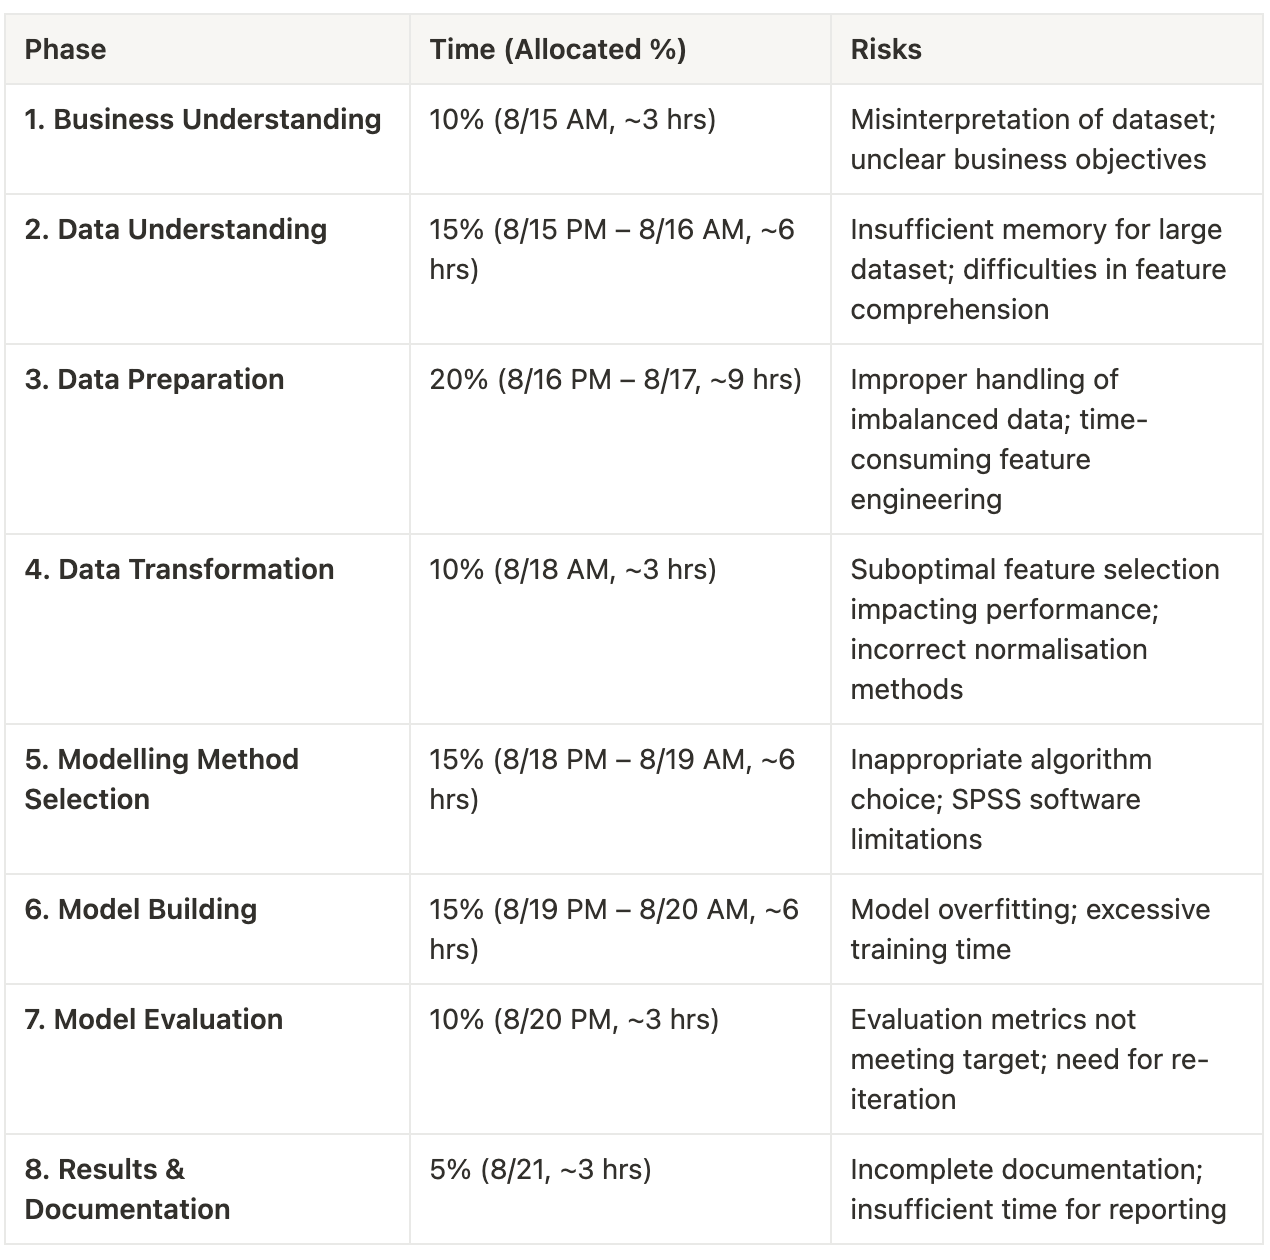
\includegraphics[width=0.9\columnwidth]{table2.jpg}
\vspace{0.2cm}

Table 2: Project Timeline and Risk Assessment
\end{center}

\vspace{0.3cm}

\section{Data Understanding}
\subsection{Collecting Initial Data}

\textbf{Data Source}

This project uses the PaySim synthetic dataset, which is publicly available on the Kaggle open data platform \cite{paysim2024}. The dataset was generated by a mobile money simulator designed to mimic real-world financial transaction environments. It contains a \textbf{total of 6,362,620 transaction records}, covering a 30-day activity period.

\textbf{Data Collection Method}

The data collection process is straightforward, aiming to analyze the original and unmodified dataset in its entirety:

\begin{enumerate}
\item \textbf{Download the original dataset:} The complete CSV archive file (paysim1.zip) was downloaded directly from the Kaggle platform and extracted to obtain the \\PS\_20174392719\_1491204439457\_log.csv file.
\item \textbf{Directly load the full dataset:} In IBM SPSS Modeler, the ``Variable File'' node from the Source palette was used to connect directly to the extracted CSV file. This operation loaded all 6.36 million records at once into the data stream for analysis, without any preliminary sampling. This ensures that all subsequent analyses are based on the most complete and original dataset.
\end{enumerate}

\vspace{0.3cm}

\begin{center}
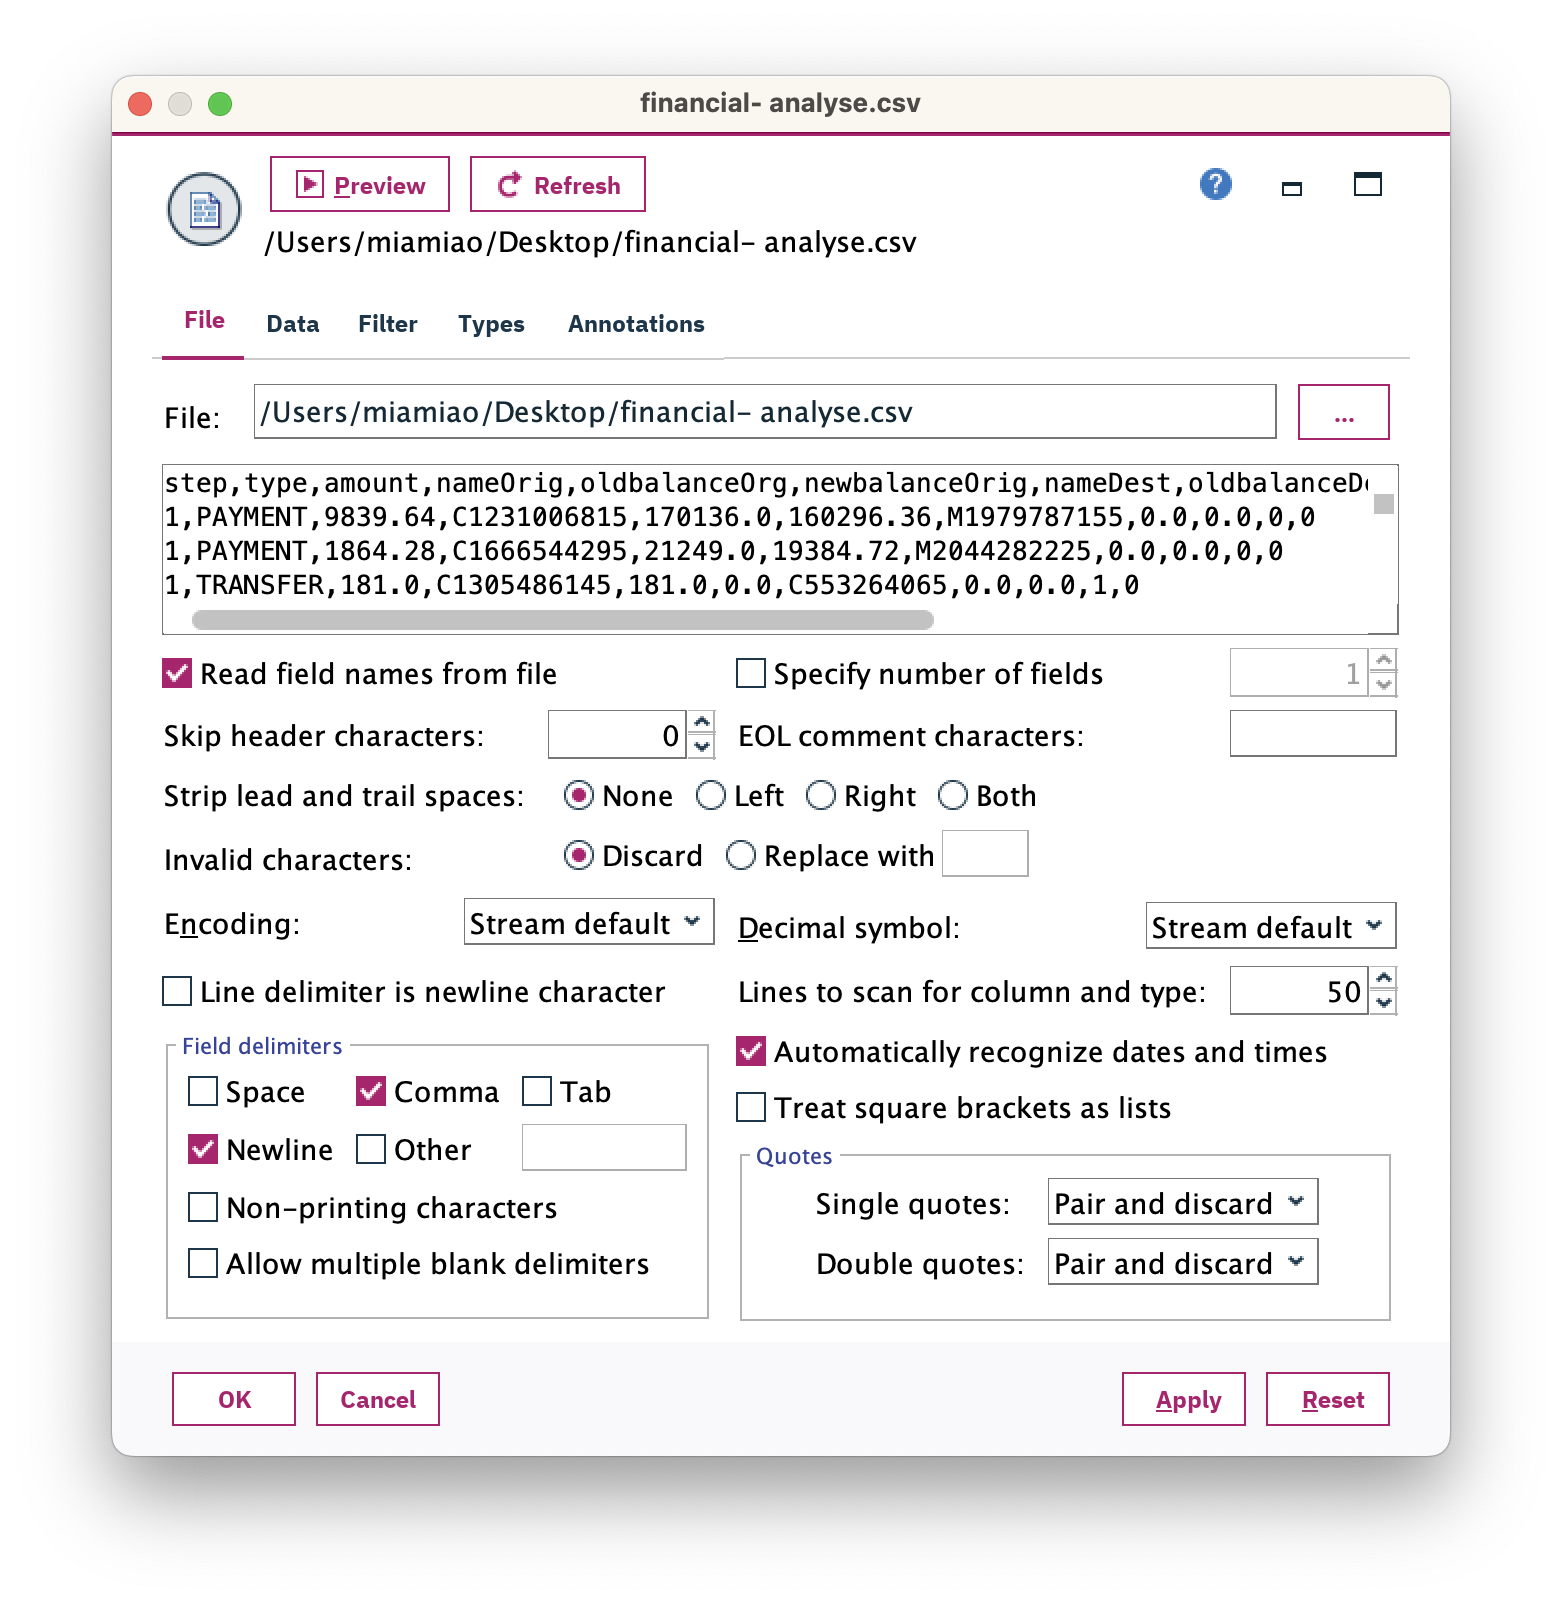
\includegraphics[width=0.9\columnwidth]{2.1.png}
\vspace{0.2cm}

Figure 2.1: Loading the complete CSV dataset directly using the ``Variable File'' node
\end{center}

\vspace{0.3cm}

\textbf{Challenges and Solutions in Data Collection}

During the initial data integration phase, I identified a critical issue: the original dataset was too large to be handled by conventional tools such as Excel. Excel has a practical row limit of approximately one million, while the dataset contained over 6.3 million records. Attempting to open it in Excel would result in incomplete loading or software crashes.

To address this, I leveraged the professional data-handling capabilities of IBM SPSS Modeler. SPSS Modeler is designed to process large-scale datasets efficiently. By using the Variable File node, I was able to seamlessly load the entire dataset into memory or process it in server mode, completely bypassing the row-limit restrictions of common office software. This ensured both the integrity and accuracy of the analysis.

\subsection{Describing Data}

\textbf{Data Format and Volume}

Based on the data audit results in IBM SPSS Modeler, the dataset has the following characteristics:

\begin{itemize}
\item \textbf{Format}: CSV file, UTF-8 encoding
\item \textbf{Total Records}: 6,362,620 transactions
\item \textbf{Number of Features}: 11 fields
\item \textbf{Completeness}: 100\% field completeness, 100\% record completeness
\item \textbf{Data Quality}: No missing values, nulls, or anomalous blanks
\end{itemize}

\textbf{Field Roles and Measurement Level Definition}

Before conducting exploratory analysis, I first used the Type node in SPSS Modeler to check and define the dataset's metadata. This step ensures that each field is correctly interpreted and that their roles in subsequent modeling are clearly specified. Key configurations are as follows:

\sloppy
\begin{itemize} 
\item \textbf{Target}: The isFraud field was explicitly set as the target, as it is the variable to be predicted in this project.
\item \textbf{Input}: Fields such as step, type, amount, oldbalanceOrig, newbalanceOrig, oldbalanceDest, and newbalanceDest were set as inputs, serving as predictive features for the model.
\item \textbf{None}: nameOrig and nameDest represent unique account IDs, which lack generalizable predictive power. Their roles were set to none, meaning they are excluded from the modeling process.
\item \textbf{Measurement Level Adjustment}: Both isFraud and isFlaggedFraud were verified and corrected to flag measurement level, to accurately reflect their binary nature.
\end{itemize}
\fussy

\vspace{0.3cm}

\begin{center}
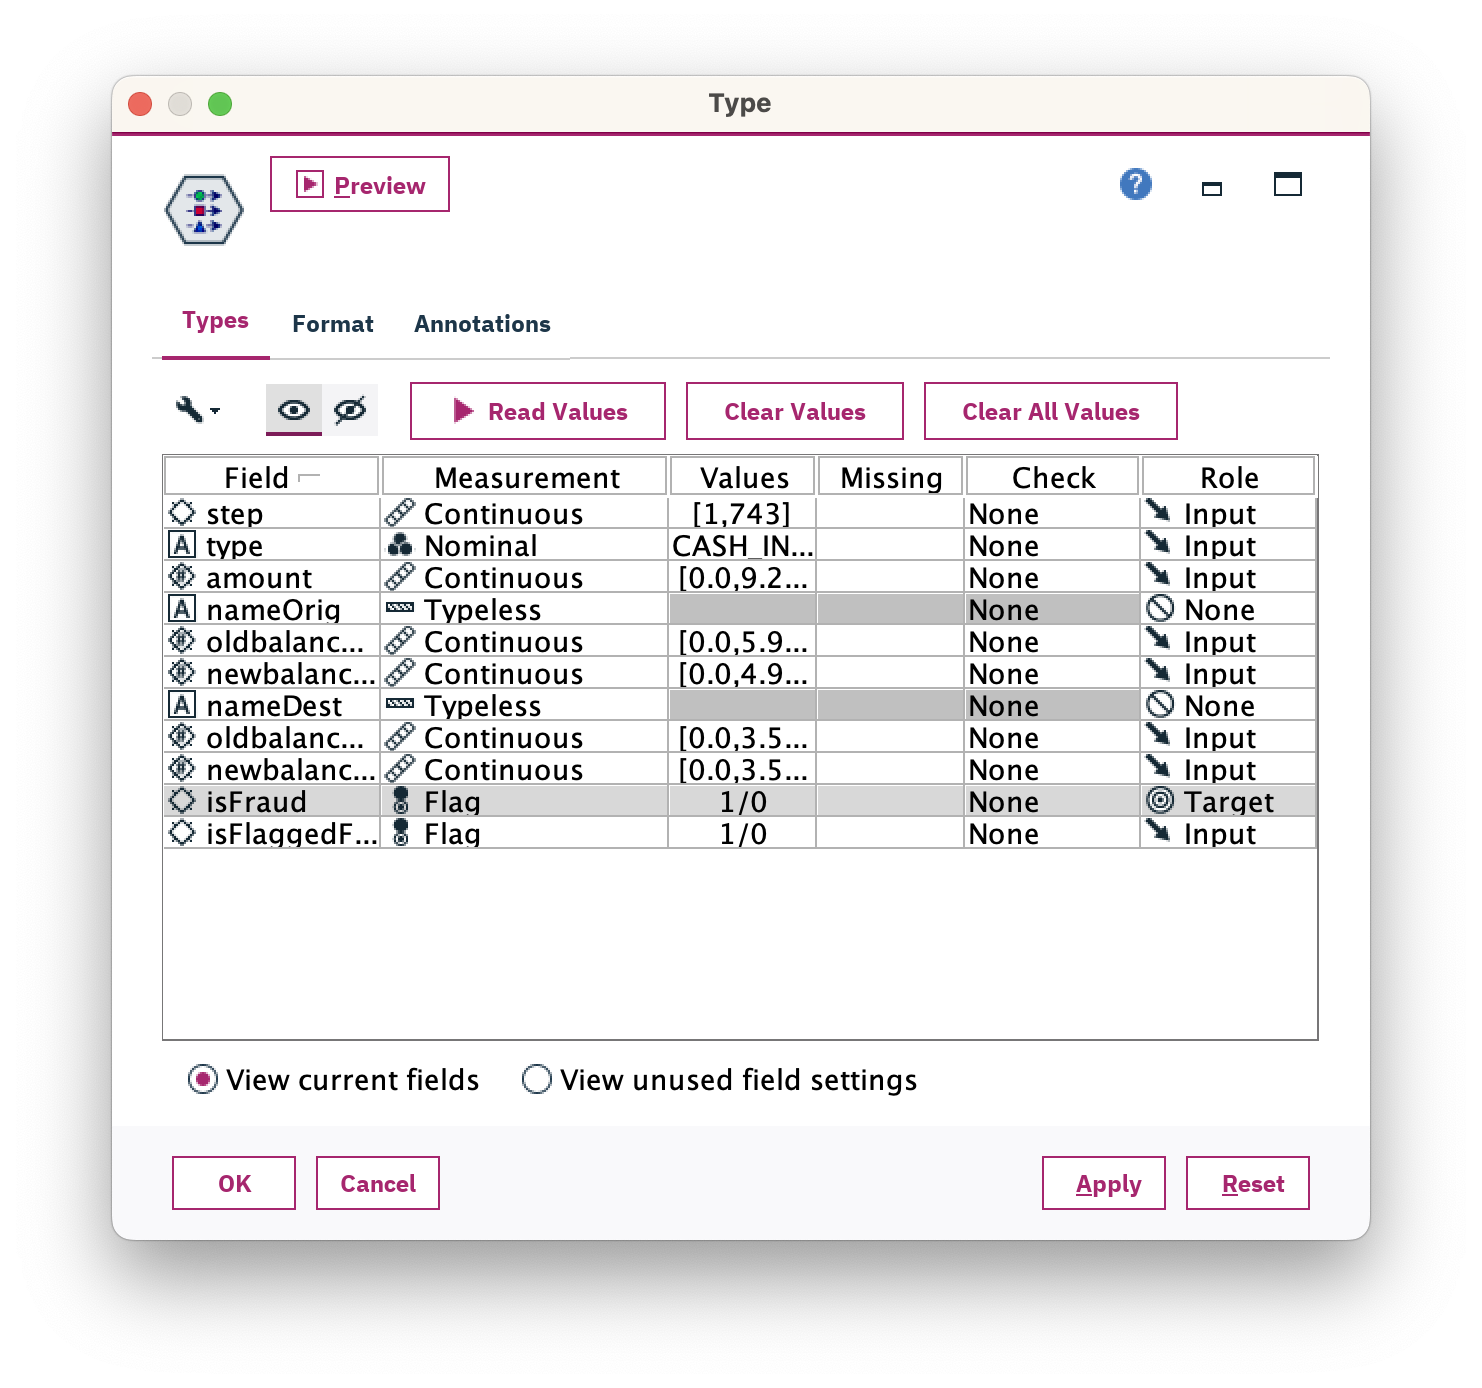
\includegraphics[width=0.9\columnwidth]{2.2.1.png}
\vspace{0.2cm}

Figure 2.2.1: Configuration of the ``Type'' node in IBM SPSS Modeler
\end{center}

\vspace{0.3cm}


\textbf{Field Detailed Description}

Based on the results of the SPSS Modeler data audit, the dataset contains the following fields:
\vspace{0.3cm}

\begin{center}
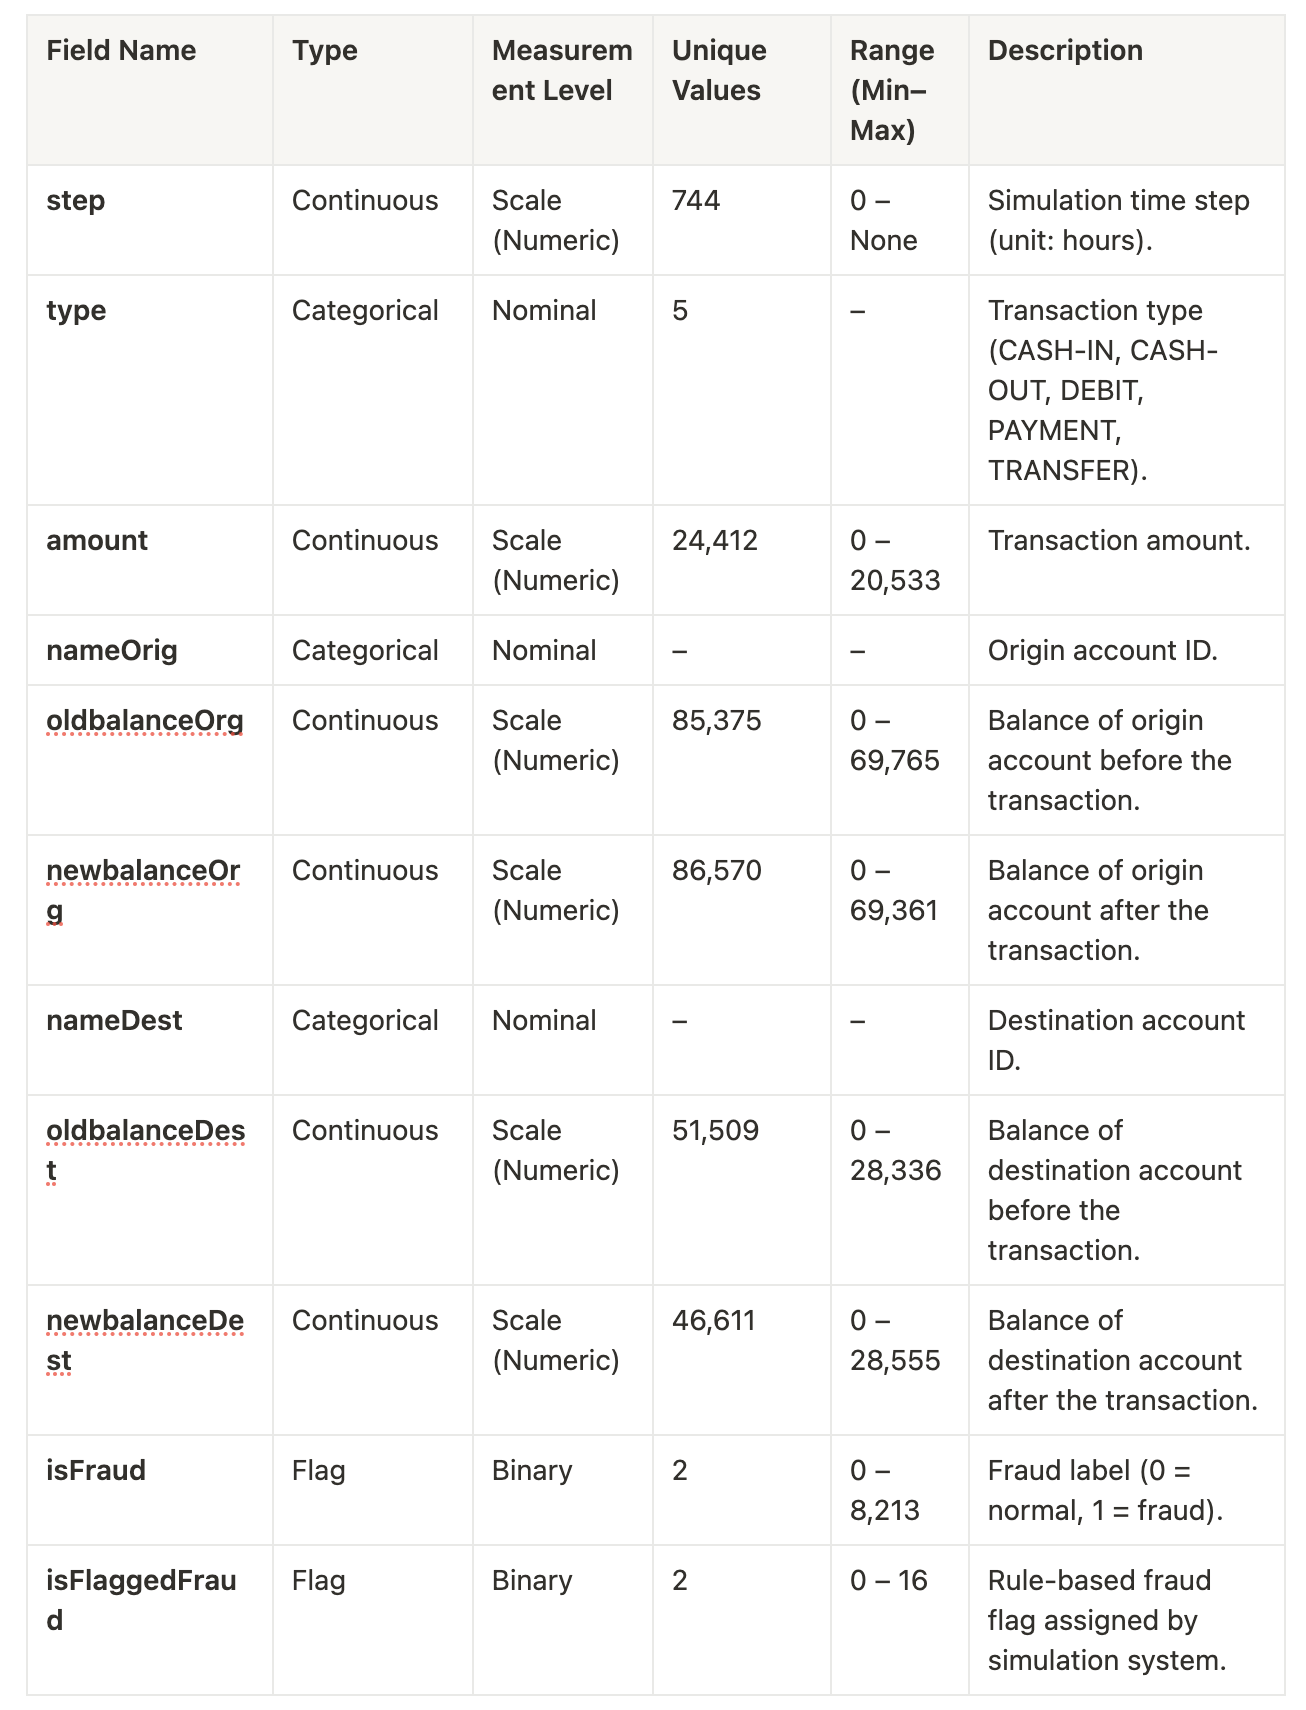
\includegraphics[width=0.9\columnwidth]{table3.jpg}
\vspace{0.2cm}

Table 3: Data Audit Results Statistics
\end{center}

\vspace{0.3cm}

\begin{center}
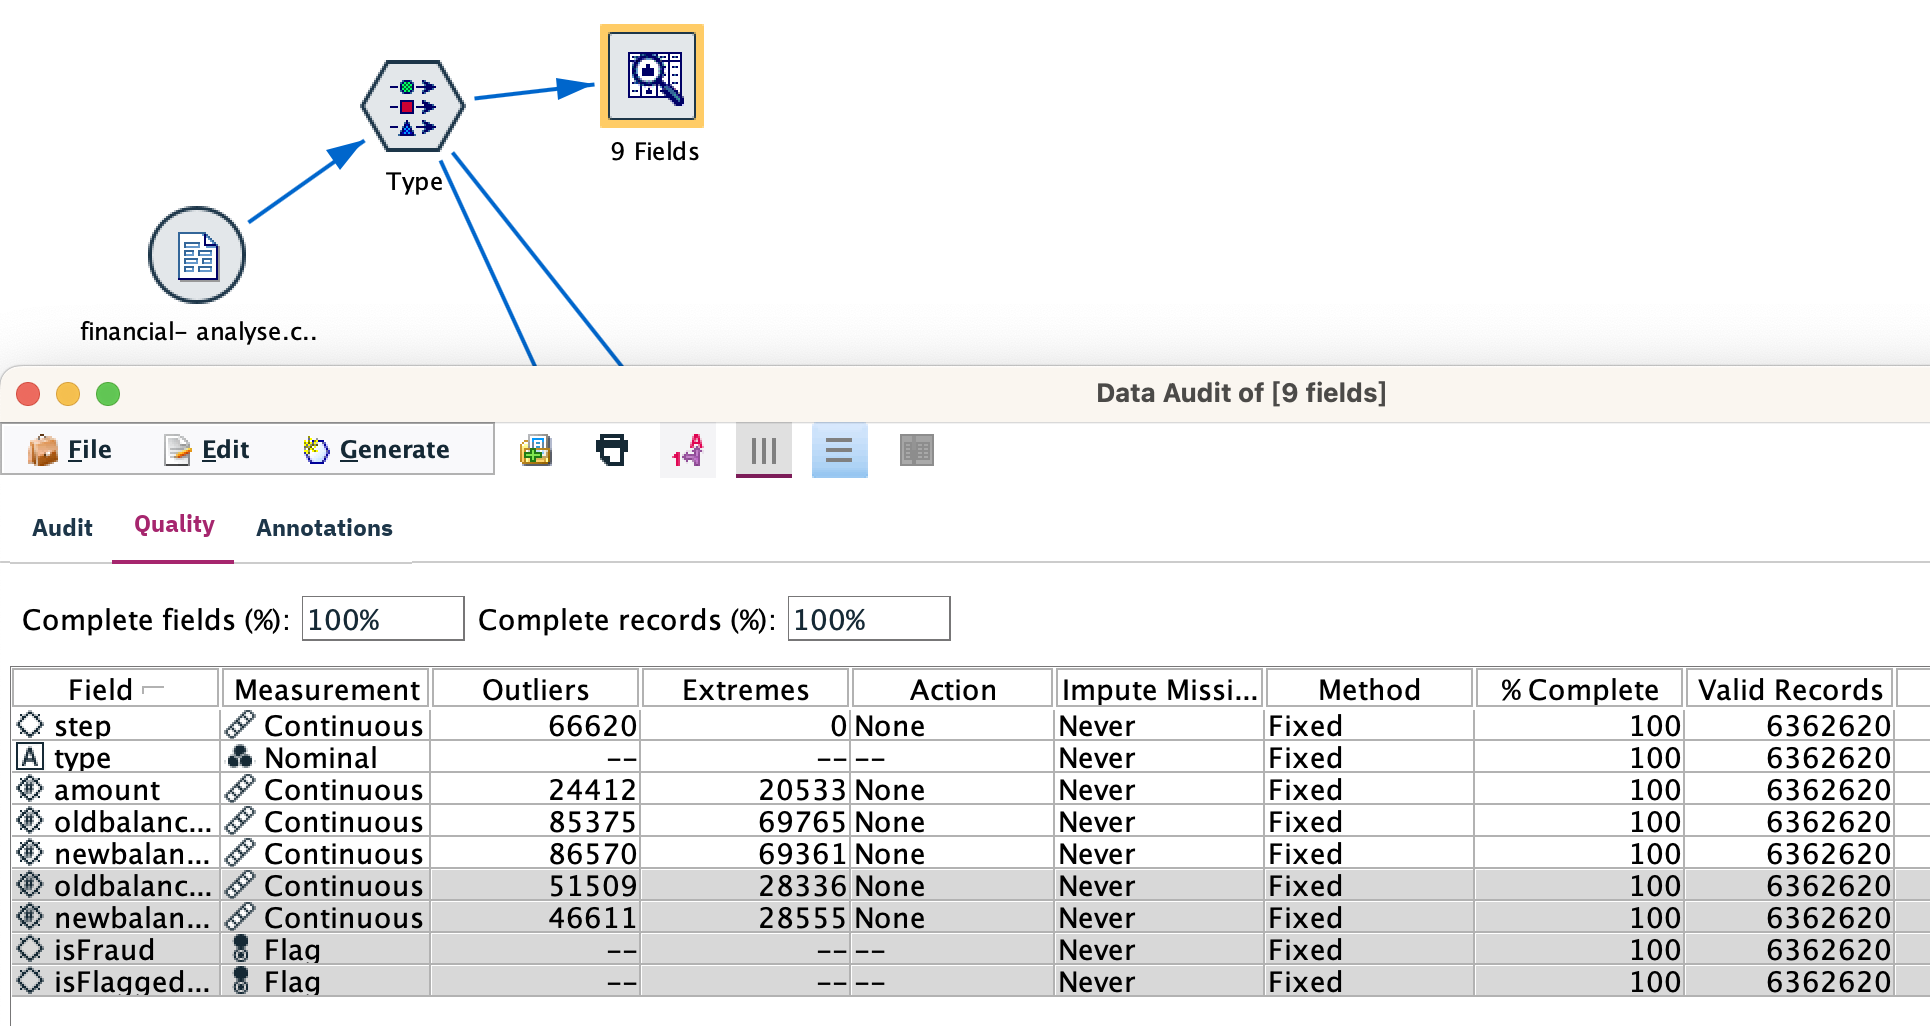
\includegraphics[width=0.9\columnwidth]{2.2.2.png}
\vspace{0.2cm}

Figure 2.2.2: Field Detailed Description
\end{center}

\vspace{0.3cm}

\textbf{Surface Feature Analysis}

\textbf{Data Distribution Characteristics:}

\begin{itemize}
\item \textbf{Transaction type distribution}: 5 types (PAYMENT, TRANSFER, CASH\_OUT, DEBIT, CASH\_IN)

\item \textbf{Extremely imbalanced}:
    \begin{itemize}
    \item Normal transactions: 6,354,407 (99.87\%)
    \item Fraudulent transactions: 8,213 (0.13\%)
    \item System-flagged fraud: only 16 (0.0003\%)
    \end{itemize}

\item \textbf{Amount feature}: 24,412 distinct values, indicating transaction diversity

\item \textbf{Account features}: Large number of unique balance change values for both origin and destination accounts, reflecting the complexity of real transactions
\end{itemize}

\subsection{Data Exploration}
According to the data mining process requirements, the core task of this stage is to gain a deep understanding of data characteristics through powerful visualization methods, to uncover patterns, and to communicate these findings clearly so as to provide explicit guidance for subsequent data preparation.

I used IBM SPSS Modeler's visualization functions (\cite{ibm_modeler_docs}), focusing on exploring the relationship between transaction type (type) and fraudulent behavior (isFraud).

\subsubsection{Overall Distribution of Transaction Types}

First, I examined the overall distribution of the five transaction types in the dataset. Using the charts generated by the Data Audit node, I produced the following distribution bar chart.

\vspace{0.3cm}

\begin{center}
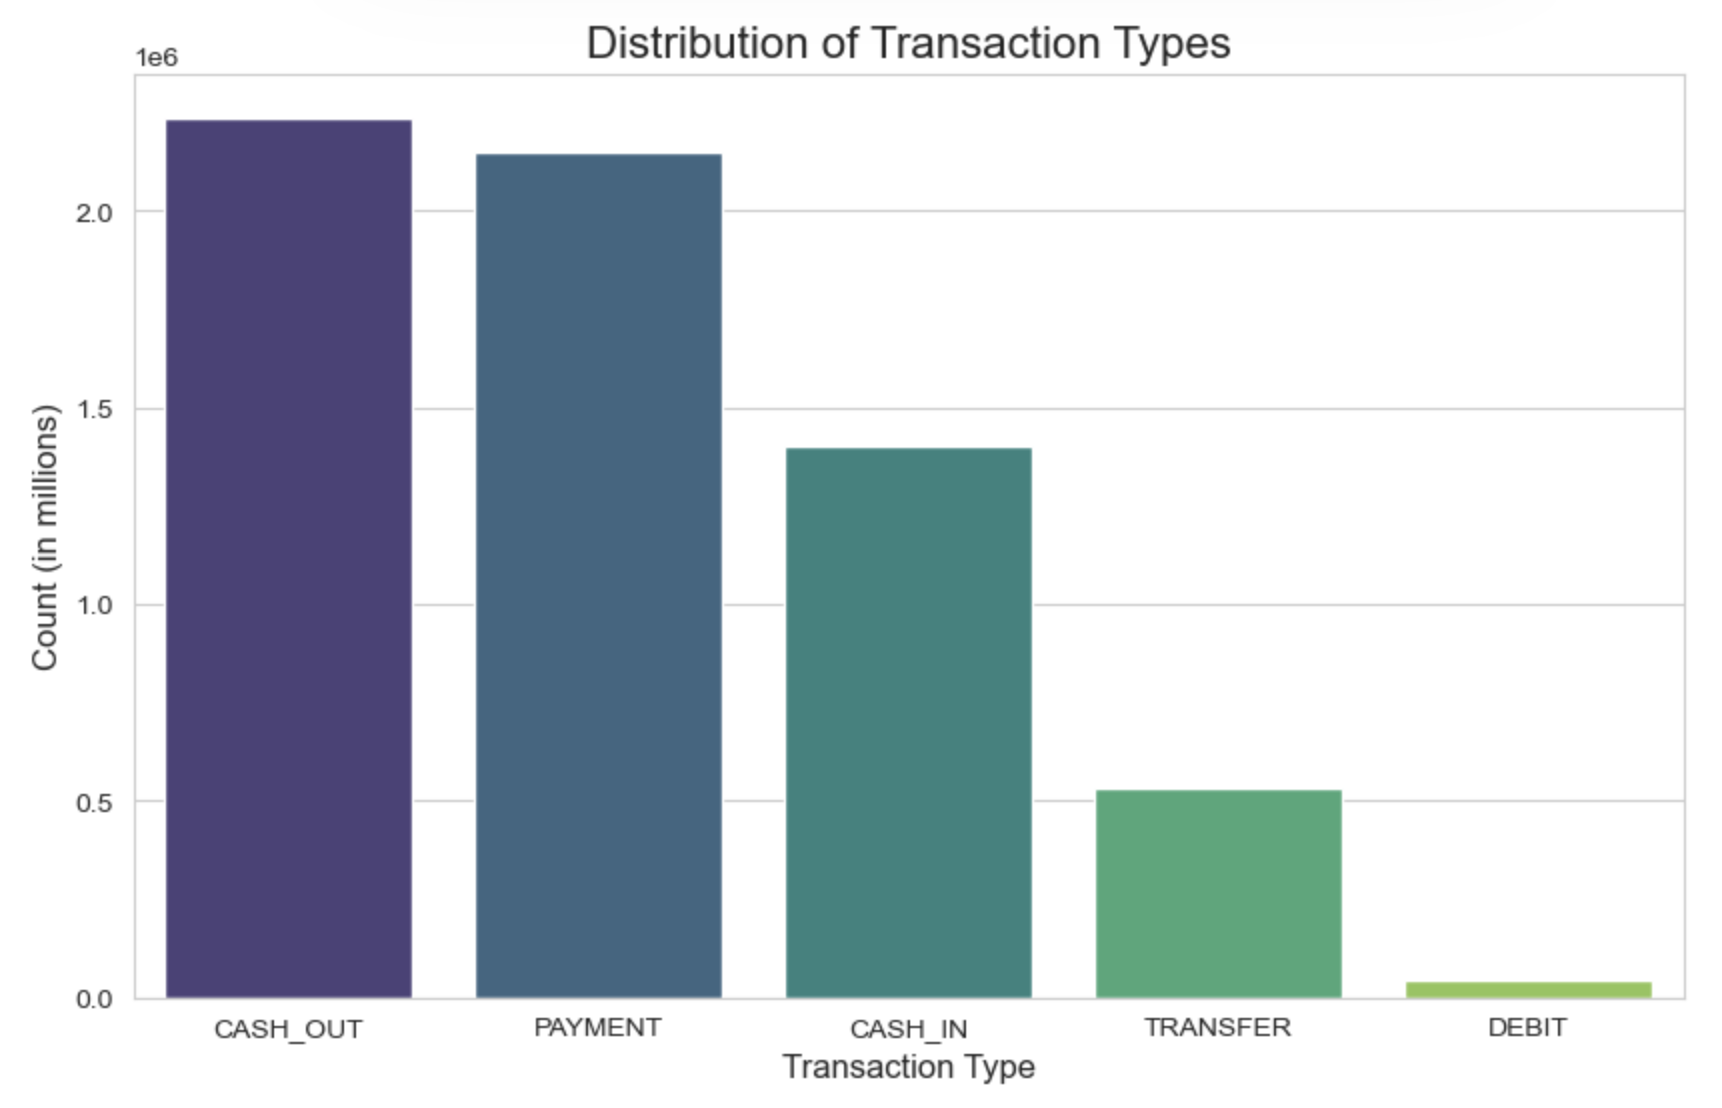
\includegraphics[width=0.9\columnwidth]{2.3.1.png}
\vspace{0.2cm}

Figure 2.3.1: Bar Chart of Transaction Type Distribution
\end{center}

\vspace{0.3cm}

From the figure above, it is clear that CASH\_OUT (withdrawal) and PAYMENT (payment) are the two most frequent transaction types in the dataset, accounting for the vast majority of transaction records.

After understanding the overall distribution, I further explored which transaction types are directly associated with actual fraudulent behavior. I used the ``Matrix'' node, setting type as the primary analysis field and outputting results with the isFraud field.

\vspace{0.3cm}

\begin{center}
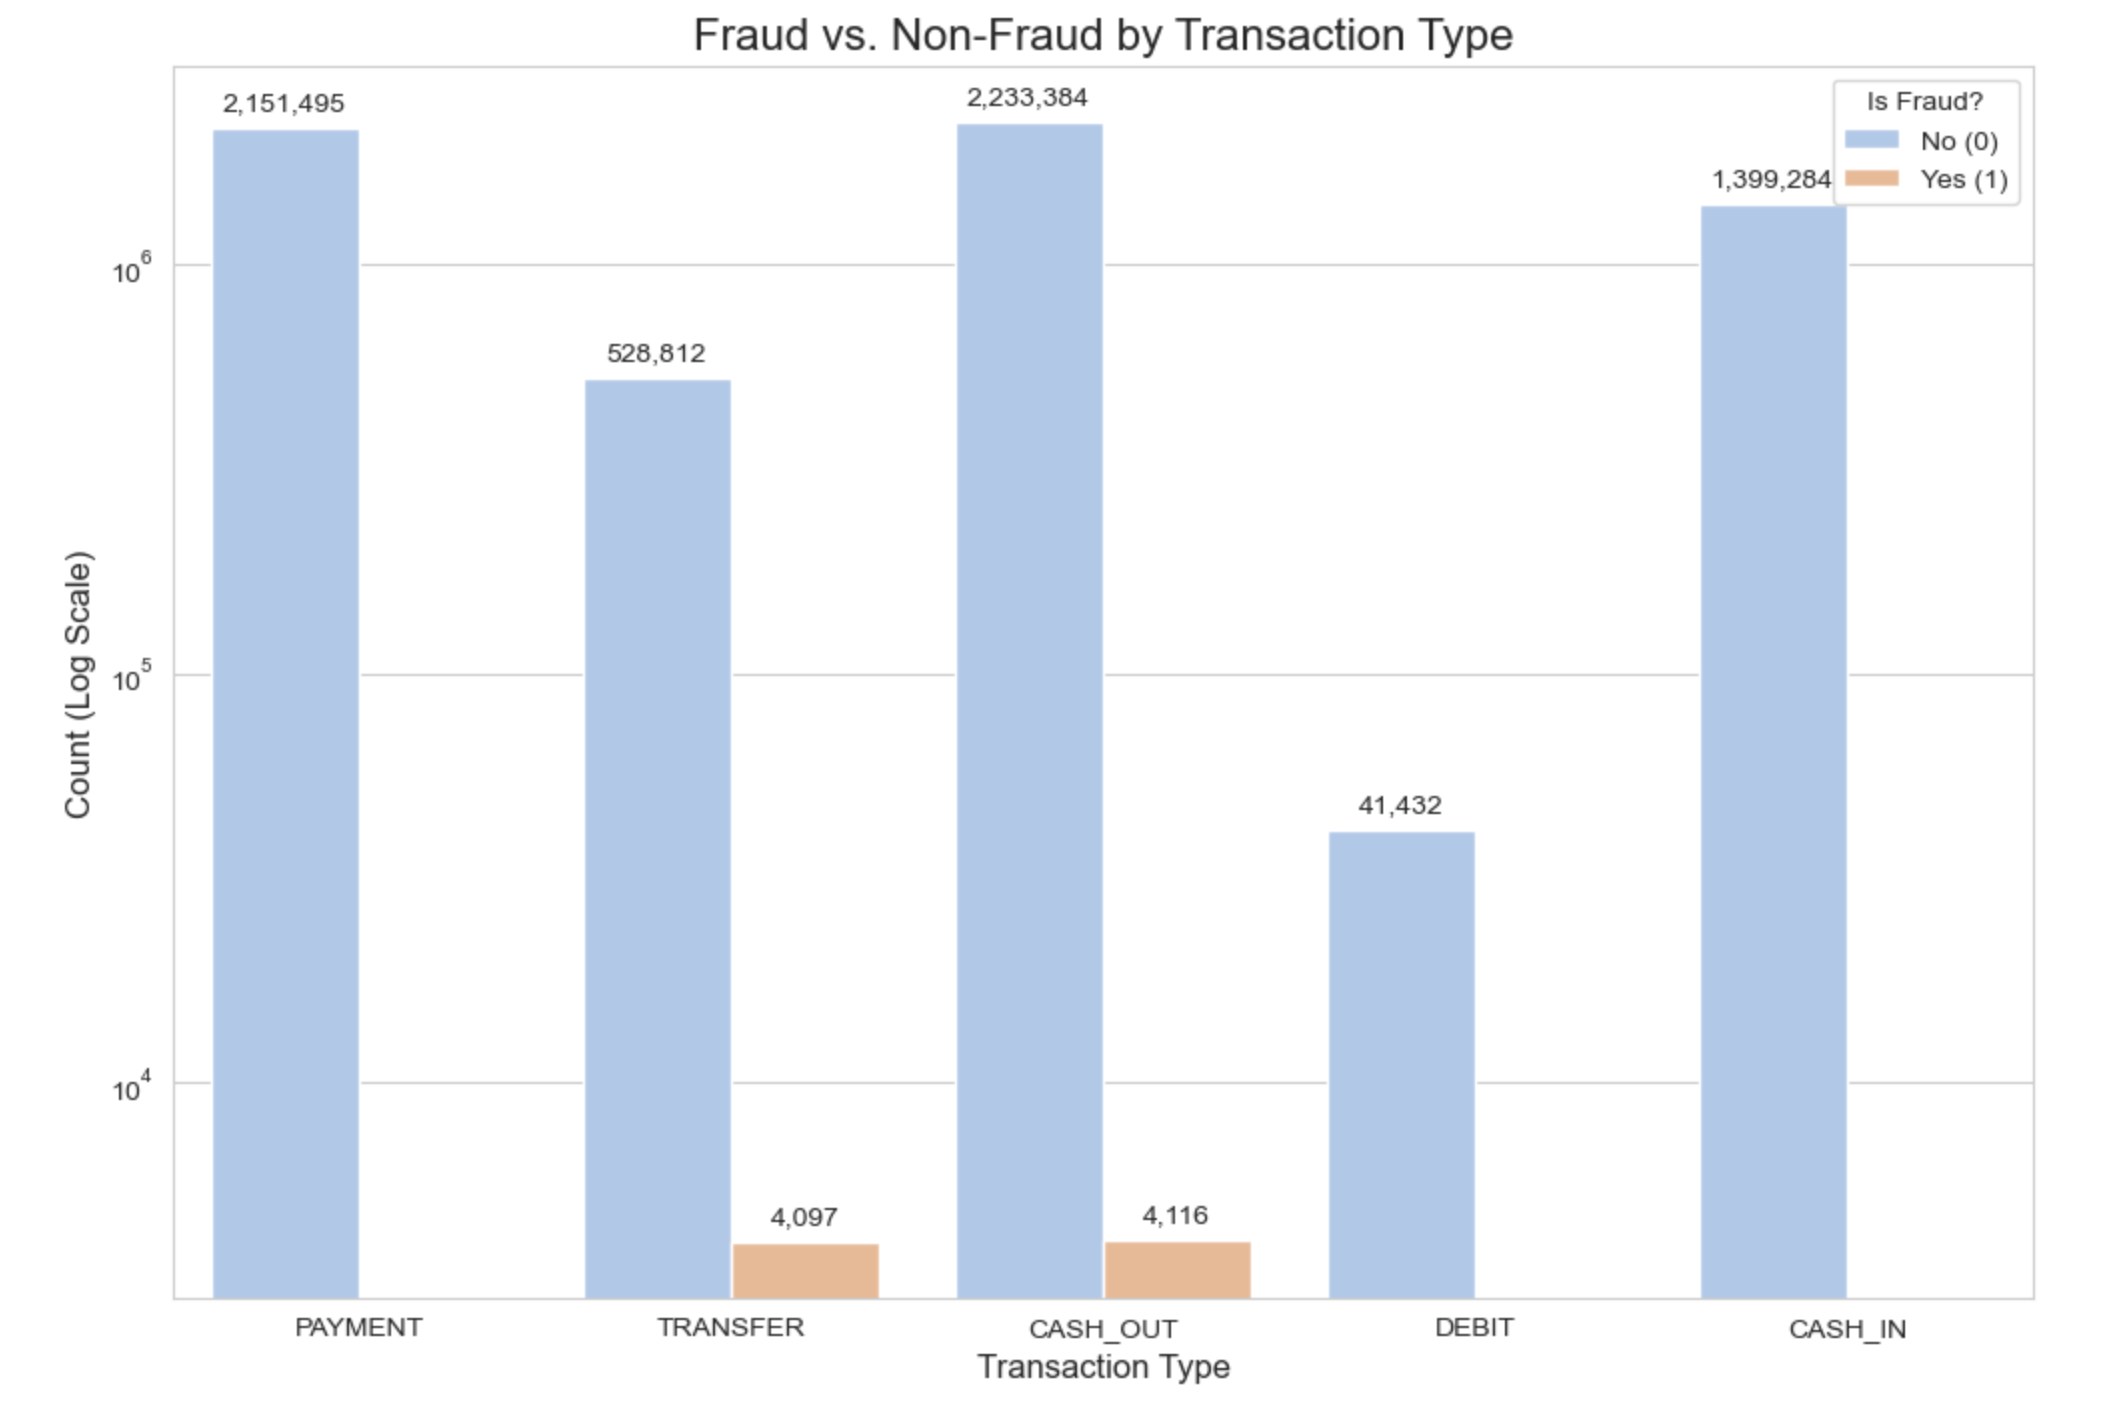
\includegraphics[width=0.9\columnwidth]{2.3.2.png}
\vspace{0.2cm}

Figure 2.3.2: Distribution of Actual Fraudulent Transactions (isFraud) and System-Flagged Fraudulent Transactions (isFlaggedFraud) by Transaction Type
\end{center}

\vspace{0.3cm}

The figure above reveals the first key insight from this exploration: records representing actual fraudulent behavior (isFraud = 1.00) only appear in the CASH\_OUT and TRANSFER transaction types. In total, there are 8,213 genuine fraudulent transactions.

Next, I evaluated the effectiveness of the dataset's built-in business rules (the isFlaggedFraud field) in detecting fraud. Using the same method, I observed the distribution of the isFlaggedFraud field across different transaction types.

The results are striking:

Among all 6.36 million transactions, those flagged as fraud by the system rules (isFlaggedFraud = 1.00) account for only 16 transactions.

When compared with the 8,213 genuine fraudulent transactions discovered in the previous step, this leads to the most critical conclusion of this exploration: the current rule-based fraud detection system is highly ineffective, with a detection rate of only (16 / 8213) $\approx$ 0.19\%, missing more than 99.8\% of actual fraud cases.

This finding highlights the severe limitations of the existing system and underscores the necessity and urgency of introducing machine learning to build a smarter and more comprehensive fraud detection model.

\subsection{Verifying Data Quality}
    
    After gaining an initial structural understanding of the data, in this stage I conducted a rigorous verification of data quality. By running the ``Data Audit'' node in IBM SPSS Modeler, I was able to perform an in-depth assessment across multiple dimensions, including completeness, consistency, and data patterns.
    
\subsubsection{Data Integrity Check}
    
    The first conclusion from the data audit report is that the dataset demonstrates an exceptionally high level of integrity.

\vspace{0.3cm}

\begin{center}
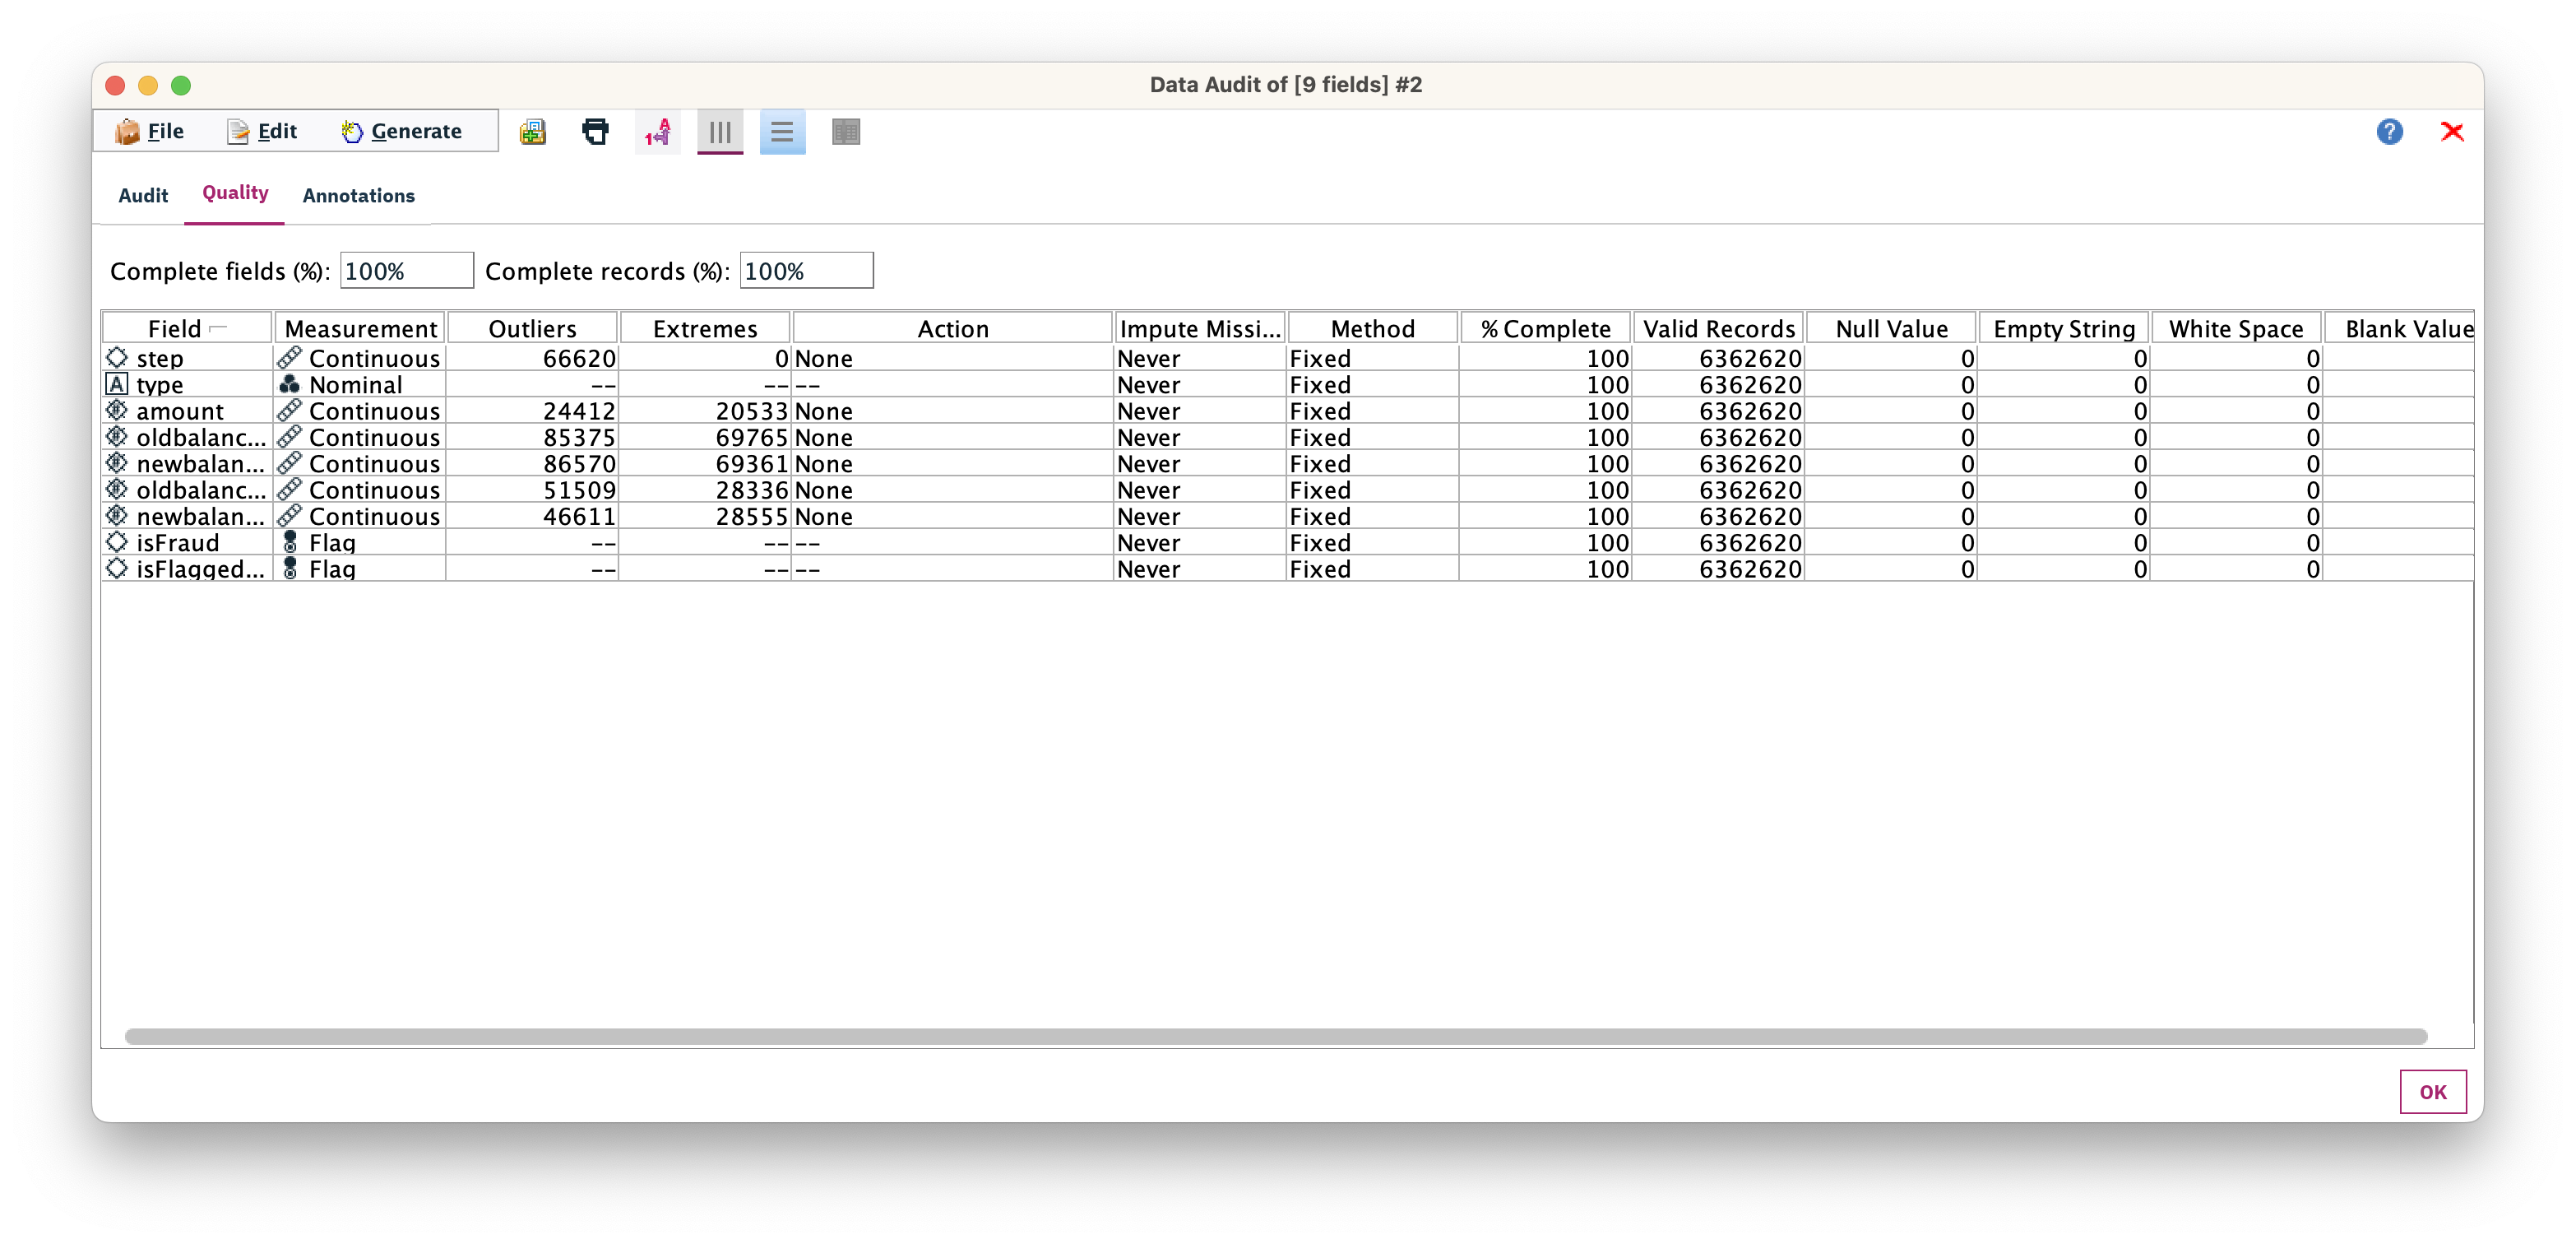
\includegraphics[width=0.9\columnwidth]{2.4.1.png}
\vspace{0.2cm}

Figure 2.4.1: Overview of Field Quality in the Data Audit Report
\end{center}

\vspace{0.3cm}

As shown in the report above, across all 6,362,620 records, the Missing and Nulls values for all 11 fields are both zero, with an effective rate of 100\%. This is an ideal situation, meaning that in the subsequent data preparation stage, I do not need to spend additional effort on complex missing-value imputation tasks.

\subsubsection{Key Data Quality Pattern Analysis}

Beyond completeness, the data audit report also revealed two data quality patterns that are critical for subsequent modeling:

\begin{itemize}
\item \textbf{1. Severe Class Imbalance in the Target Field}: This is the most important characteristic identified in this analysis. By examining the statistics of the target field isFraud, I found that a serious class imbalance exists.

\vspace{0.3cm}

\begin{center}
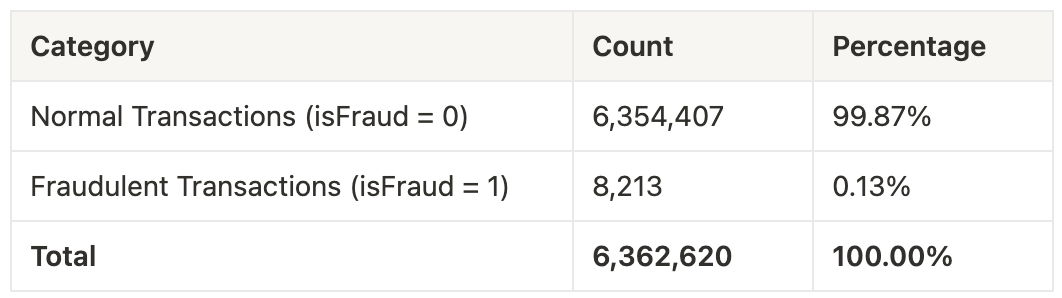
\includegraphics[width=0.9\columnwidth]{table4.jpg}
\vspace{0.2cm}

Table 4: Distribution of isFraud (Counts \& Percentages)
\end{center}

\vspace{0.3cm}

Such extreme imbalance is a typical characteristic and major challenge of fraud detection projects. It implies that:

\begin{itemize}
\item {Standard classification algorithms may be biased toward predicting the majority class (normal transactions), thereby overlooking the fraudulent samples that are of greatest concern.}
\item {``Accuracy'' is no longer a reliable evaluation metric.}
\end{itemize}

Therefore, in the subsequent data preparation phase, specialized techniques such as undersampling or oversampling must be applied to address this issue.

\item \textbf{2. Business Pattern in Specific Values}

The statistical summary from the Data Audit report shows that the minimum value of the receiver's balance fields (oldbalanceDest and newbalanceDest) is zero, and this occurs with high frequency.

Cross-validation with the Data Exploration phase reveals that this pattern is mainly observed in transactions where type = PAYMENT, and the receiver account nameDest usually begins with the letter \textbf{``M''}, indicating merchant IDs.

This is \textbf{not a data error} but rather a business-specific feature. It demonstrates that, when recording payments made to merchants, the system does not track the merchants' account balances. This insight is critical, as it indicates that for merchant payment transactions, the fields oldbalanceDest and newbalanceDest may not provide predictive value. This will be carefully considered in subsequent feature engineering and selection.
\end{itemize}

\subsubsection{Summary of Data Quality}

In summary, the PaySim dataset demonstrates very high data integrity, but reveals two key patterns:

\begin{itemize}
\item \textbf{Severe class imbalance} in the target variable.
\item \textbf{Business-driven absence of information} in certain fields.
\end{itemize}

\section{Data Preparation}

\subsection{Data Selection}
After gaining a comprehensive understanding of the structure and quality of the data, I proceeded to the first step of Data Preparation: Data Selection. The goal of this step is to streamline the dataset based on the key insights obtained during the data exploration stage (Section 2.3), retaining only those records and features most relevant to the fraud prediction task, thereby enhancing the efficiency and accuracy of subsequent modeling.

\subsubsection{Record Selection (Row Filtering)}
As established in Section 2.3.2, genuine fraudulent activities (isFraud = 1) occur exclusively in the CASH\_OUT and TRANSFER transaction types. All other transaction types (such as PAYMENT) are unrelated to fraud.

To precisely focus the analysis on these two critical transaction categories, I used the ``Select'' node from the Record Operation palette in IBM SPSS Modeler to filter the data stream at the record level. As shown in Figure 3.1.1, I set the following condition within the node:

\vspace{0.3cm}

\begin{center}
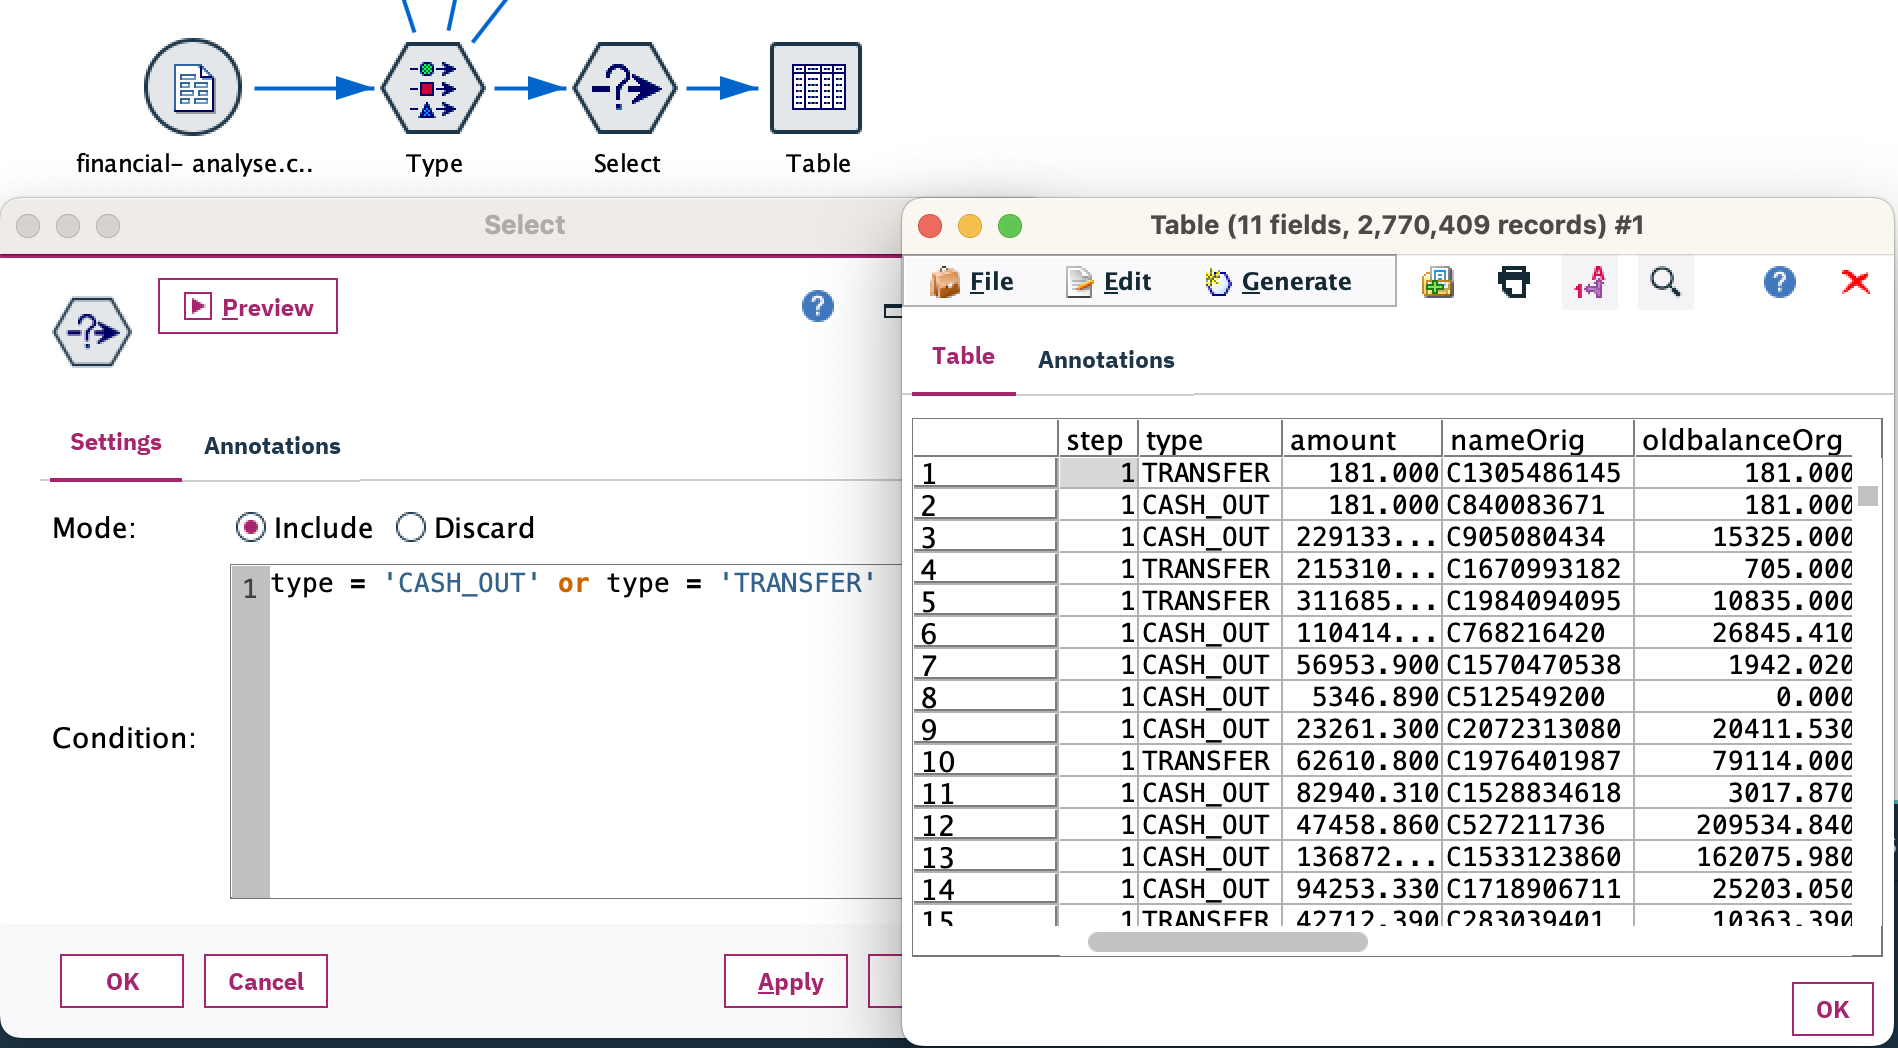
\includegraphics[width=0.9\columnwidth]{3.1.1.png}
\vspace{0.2cm}

Figure 3.1.1: Configuring conditions in the SPSS Modeler Select node to filter and retain only records belonging to the CASH\_OUT and TRANSFER transaction types that are associated with fraud.
\end{center}

\vspace{0.3cm}
This operation reduced the dataset from the original 6,362,620 records down to 2,770,409 records. Importantly, while eliminating more than 56% of irrelevant records, this step retained all 8,213 fraud cases in full, achieving an efficient yet lossless initial reduction.

\subsubsection{Feature Selection (Column Filtering)}

The 11 original features were evaluated, and the following fields were removed as they provide no benefit to model construction or could introduce noise:

\begin{itemize}
\item \textbf{nameOrig, nameDest}: These fields represent the account IDs of the sender and recipient. They are high-cardinality identifiers useful for distinguishing individual transactions, but they hold no predictive value for training a machine learning model with generalization capability.
\item \textbf{isFlaggedFraud}: As demonstrated in Section 2.3.3, this is an extremely inefficient business rule (identifying only 16 out of 8,213 fraud cases). Including it as a feature would introduce noise rather than useful information. In highly imbalanced settings, overall accuracy can be misleading\cite{he2009learning}.
\end{itemize}
    
As shown in Figure 3.1.2, I used the ``Filter'' node from the   Field Operations palette to remove these three fields from the data stream, ensuring they do not enter subsequent model training stages.

\vspace{0.3cm}

\begin{center}
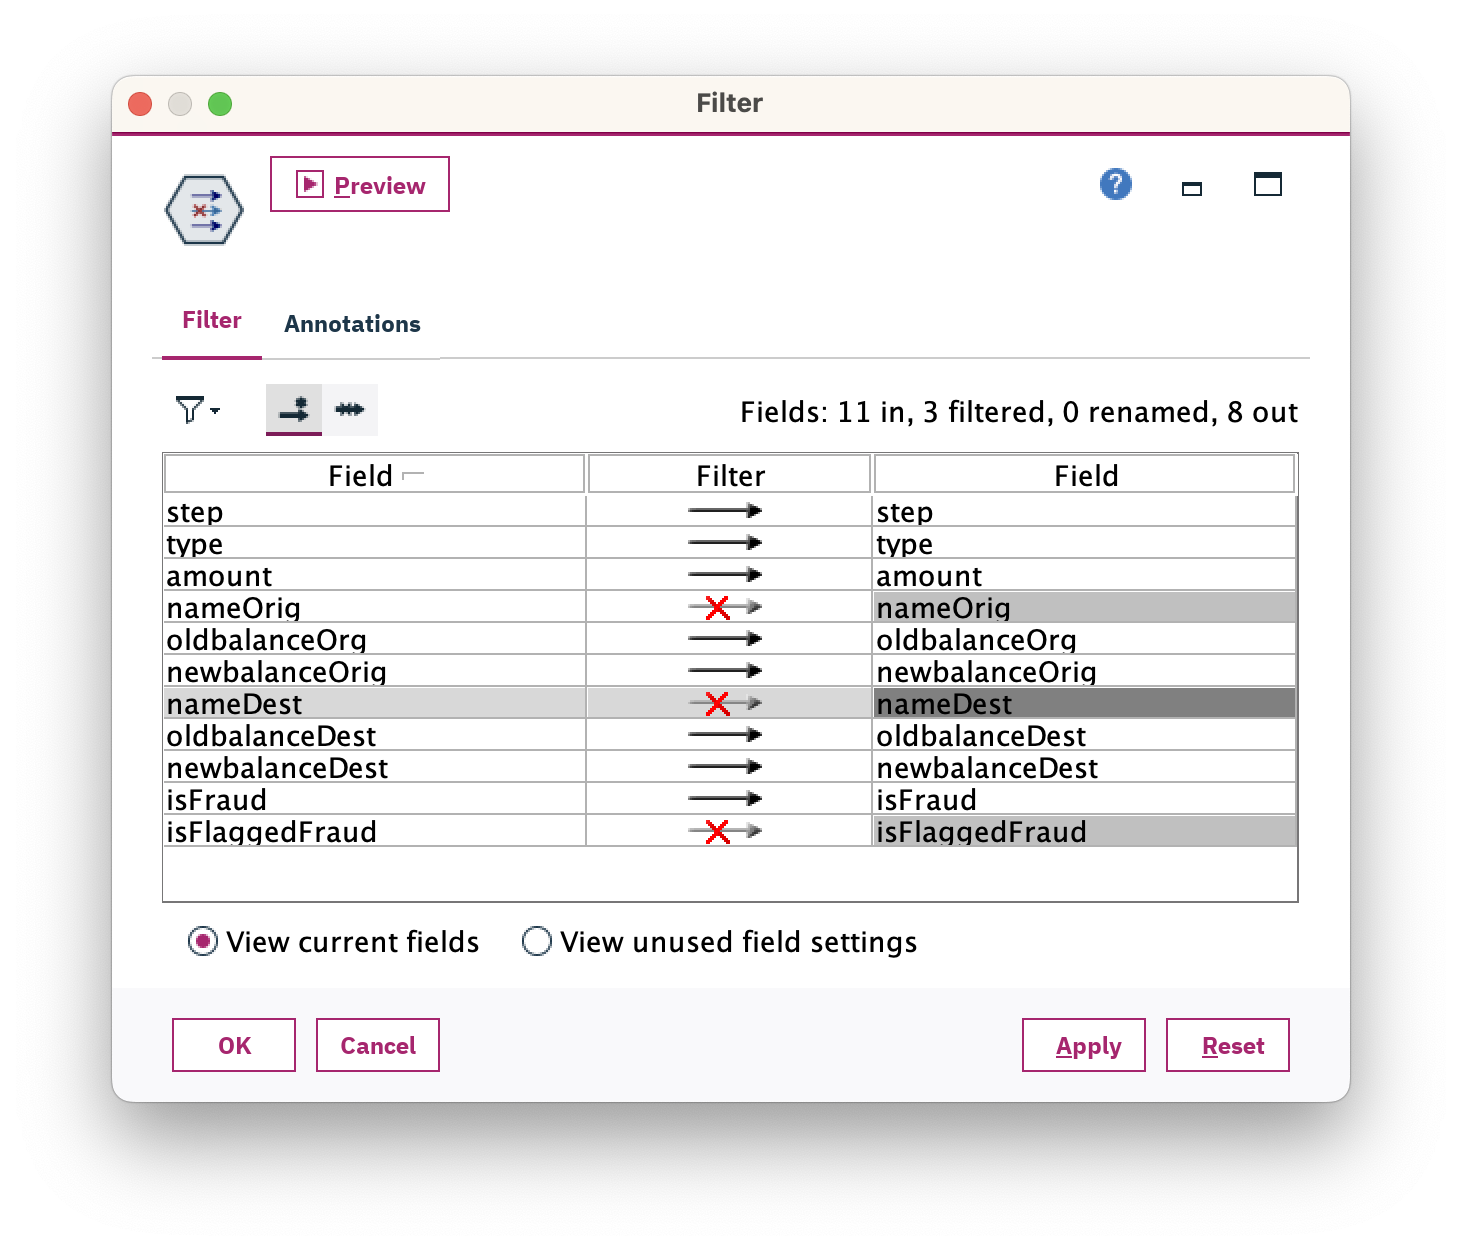
\includegraphics[width=0.9\columnwidth]{3.1.2.png}
\vspace{0.2cm}

Figure 3.1.2: Using Select and Filter nodes in SPSS Modeler for data selection.
\end{center}

\vspace{0.3cm}
Through record and feature selection, I successfully transformed a large and broad dataset into a smaller, more focused subset with a higher signal-to-noise ratio. This refined dataset lays a solid foundation for the next stages of data cleaning and transformation.

\subsection{Cleaning the Data}
    
After completing the initial data selection, I moved on to improving the \textit{cleanliness} of the dataset. The goal of data cleaning is to remove noise and irrelevant information, ensuring a high-quality dataset that can support reliable feature engineering and model training.
    
\subsubsection{Cleaning Strategy}
    
Based on the data quality assessment in Section 2.4, the dataset contains no missing values or formatting errors. Therefore, traditional cleaning tasks such as imputing missing values or correcting data types are unnecessary. Instead, the core cleaning strategy is to remove noise and irrelevant information that could hinder the fraud prediction task.
    
\subsubsection{Cleaning Operations and Rationale}
    
\begin{enumerate}
\item \textbf{Removing Noisy Records}
    \begin{itemize}
    \item \textbf{Issue Identified:} More than 56\% of the records (e.g., PAYMENT, CASH\_IN transactions) were confirmed during data exploration to be entirely unrelated to fraudulent behavior. Feeding these records into the model would not only increase computational overhead significantly but also distract the model from learning true fraud patterns. In essence, they represent ``noise.''
    \item \textbf{Cleaning Method:} As detailed in Section 3.1, I used the \textbf{Select node} to exclude these noisy records, ensuring that the dataset focuses exclusively on fraud-relevant transaction types (CASH\_OUT and TRANSFER).
    \end{itemize}
\item \textbf{Removing Redundant Features}
    \begin{itemize}
    \item \textbf{Issue Identified:} Fields such as nameOrig and nameDest (account identifiers) and isFlaggedFraud (a proven ineffective rule-based feature) provide no generalizable predictive value and may mislead the learning process.
    \item \textbf{Cleaning Method:} Using the \textbf{Filter node}, I removed these fields to eliminate redundancy and reduce the risk of introducing misleading signals into the model.
    \end{itemize}
\end{enumerate}
    
\subsubsection{Cleaning Summary}
    
This stage of cleaning centered on \textbf{removing noise and redundancy} rather than performing complex corrections. While simple in execution, it followed a key principle of data mining: \textbf{maximizing the signal-to-noise ratio}. As a result, the dataset passed to the next phase is both cleaner and more focused, ensuring that subsequent feature engineering efforts will be more effective and directly aligned with the fraud detection goal.

\subsection{Data Construction}
    
After completing data selection and cleaning, I moved into a critical stage of data preparation---\textbf{data construction}. The objective of this stage is to generate new features (or ``variables'') from the existing ones, thereby creating inputs that are both more valuable for subsequent modeling and compatible with the algorithms to be applied.
    
\subsubsection{Objective and Method of Construction}
    
The primary task in this round of feature construction was to convert the type field, originally stored in text format, into a numerical representation that machine learning models (such as logistic regression) can directly process. Without this transformation, the model would not be able to operate.
    
To achieve this in SPSS Modeler, I employed one of the core tools from the Field Operations palette, the Derive node. As shown in the figure below, I connected the Derive node immediately after the Filter node in the data stream to perform the necessary transformation.

\vspace{0.3cm}

\begin{center}
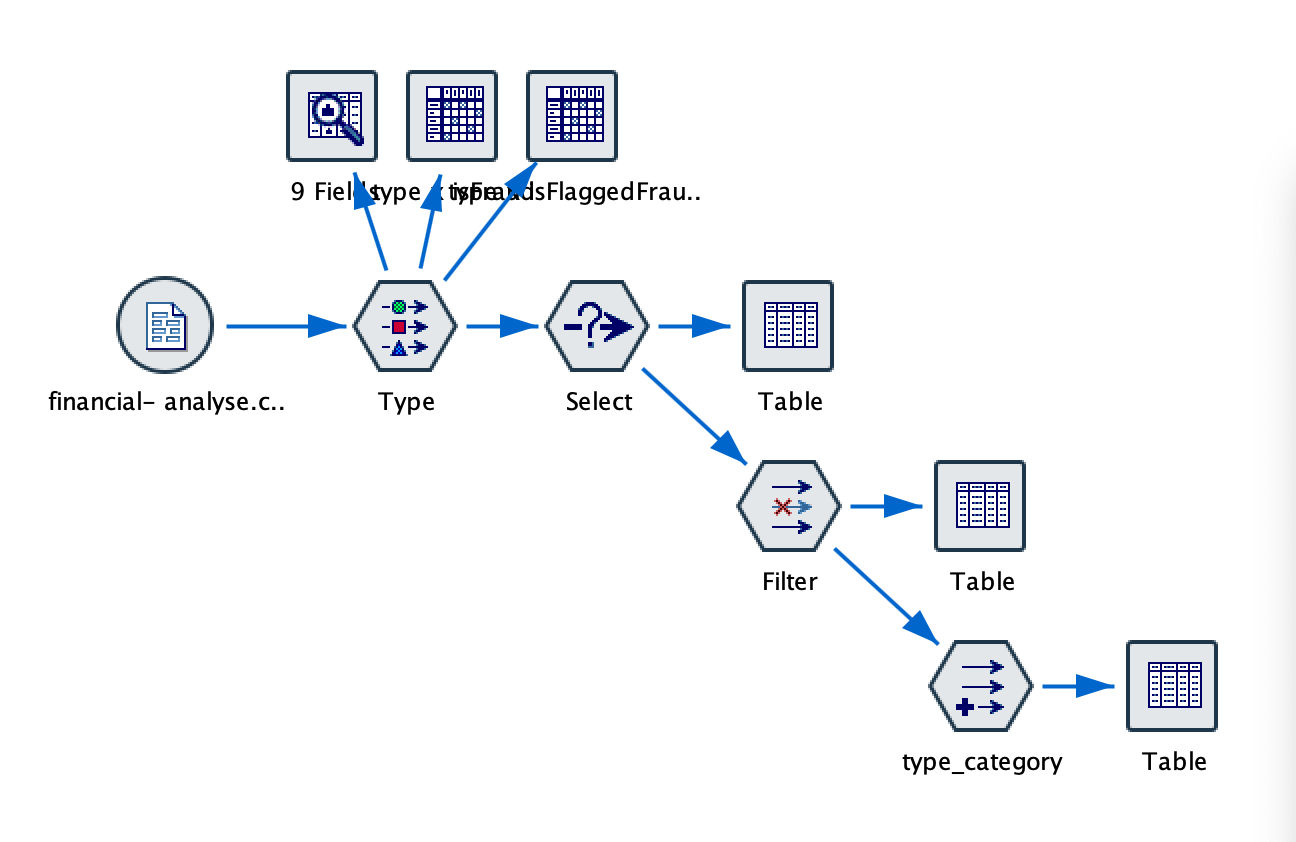
\includegraphics[width=0.9\columnwidth]{3.3.1.png}
\vspace{0.2cm}

Figure 3.3.1: Adding a Derive node to the data stream for feature construction
\end{center}

\vspace{0.3cm}

\subsubsection{ Feature Construction and Implementation}

Using the Derive node, I created a new numerical field named type\_category. The specific configuration and transformation logic are shown in Figure 3.3.2.

\vspace{0.3cm}

\begin{center}
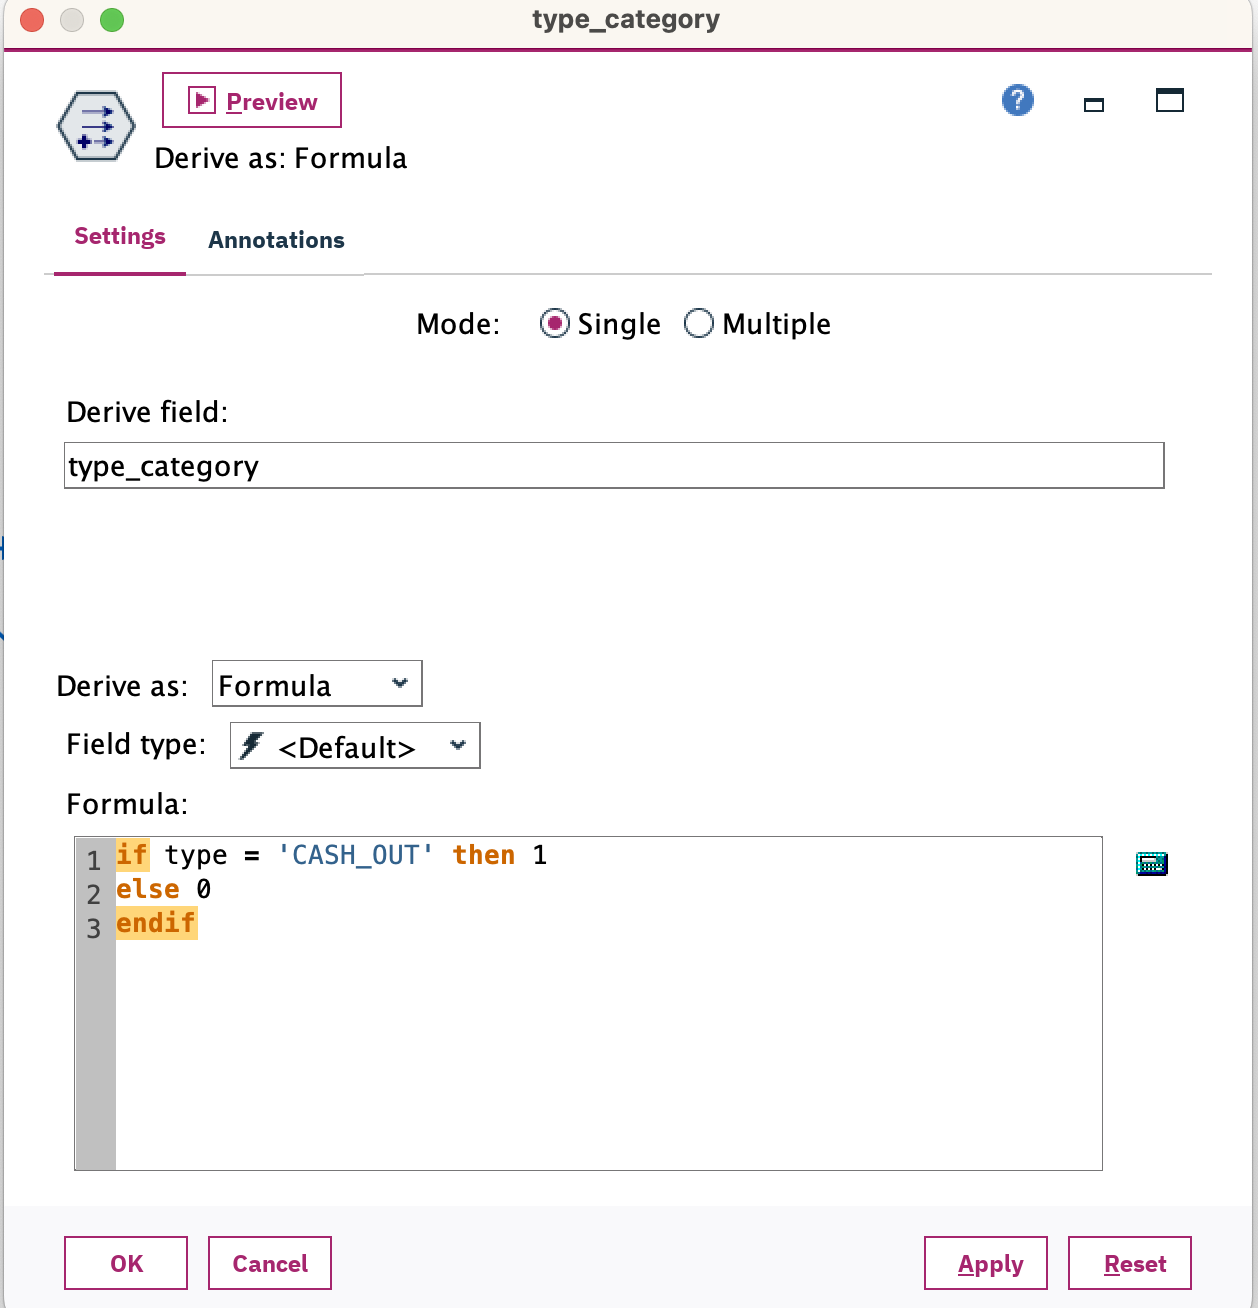
\includegraphics[width=0.9\columnwidth]{3.3.2.png}
\vspace{0.2cm}

Figure 3.3.2: Configuration of the Derive Node (Mapping type to type\_category: CASH\_OUT = 1, TRANSFER = 0)
\end{center}

\vspace{0.3cm}

I defined the following CLEM expression:

\begin{verbatim}
if type = 'CASH_OUT' then 1 else 0 endif  
\end{verbatim}

The logic of this formula is as follows:

\begin{itemize}
\item When the original type field has the value 'CASH\_OUT', the new field type\_category is assigned the value **1**.
\item In all other cases (in this filtered subset, when type = 'TRANSFER'), the new field type\_category is assigned the value **0**.
\end{itemize}

Through this simple conditional statement, I successfully converted categorical text information into a binary numerical variable with clear discriminative meaning.

\subsubsection{Validation of the Constructed Feature}

To ensure the new feature was constructed correctly, I connected a Table node immediately after the Derive node. This allowed me to preview and validate the transformation results, confirming that the type\_category field accurately reflects the intended mapping.

\begin{figure}[H]
    \centering
    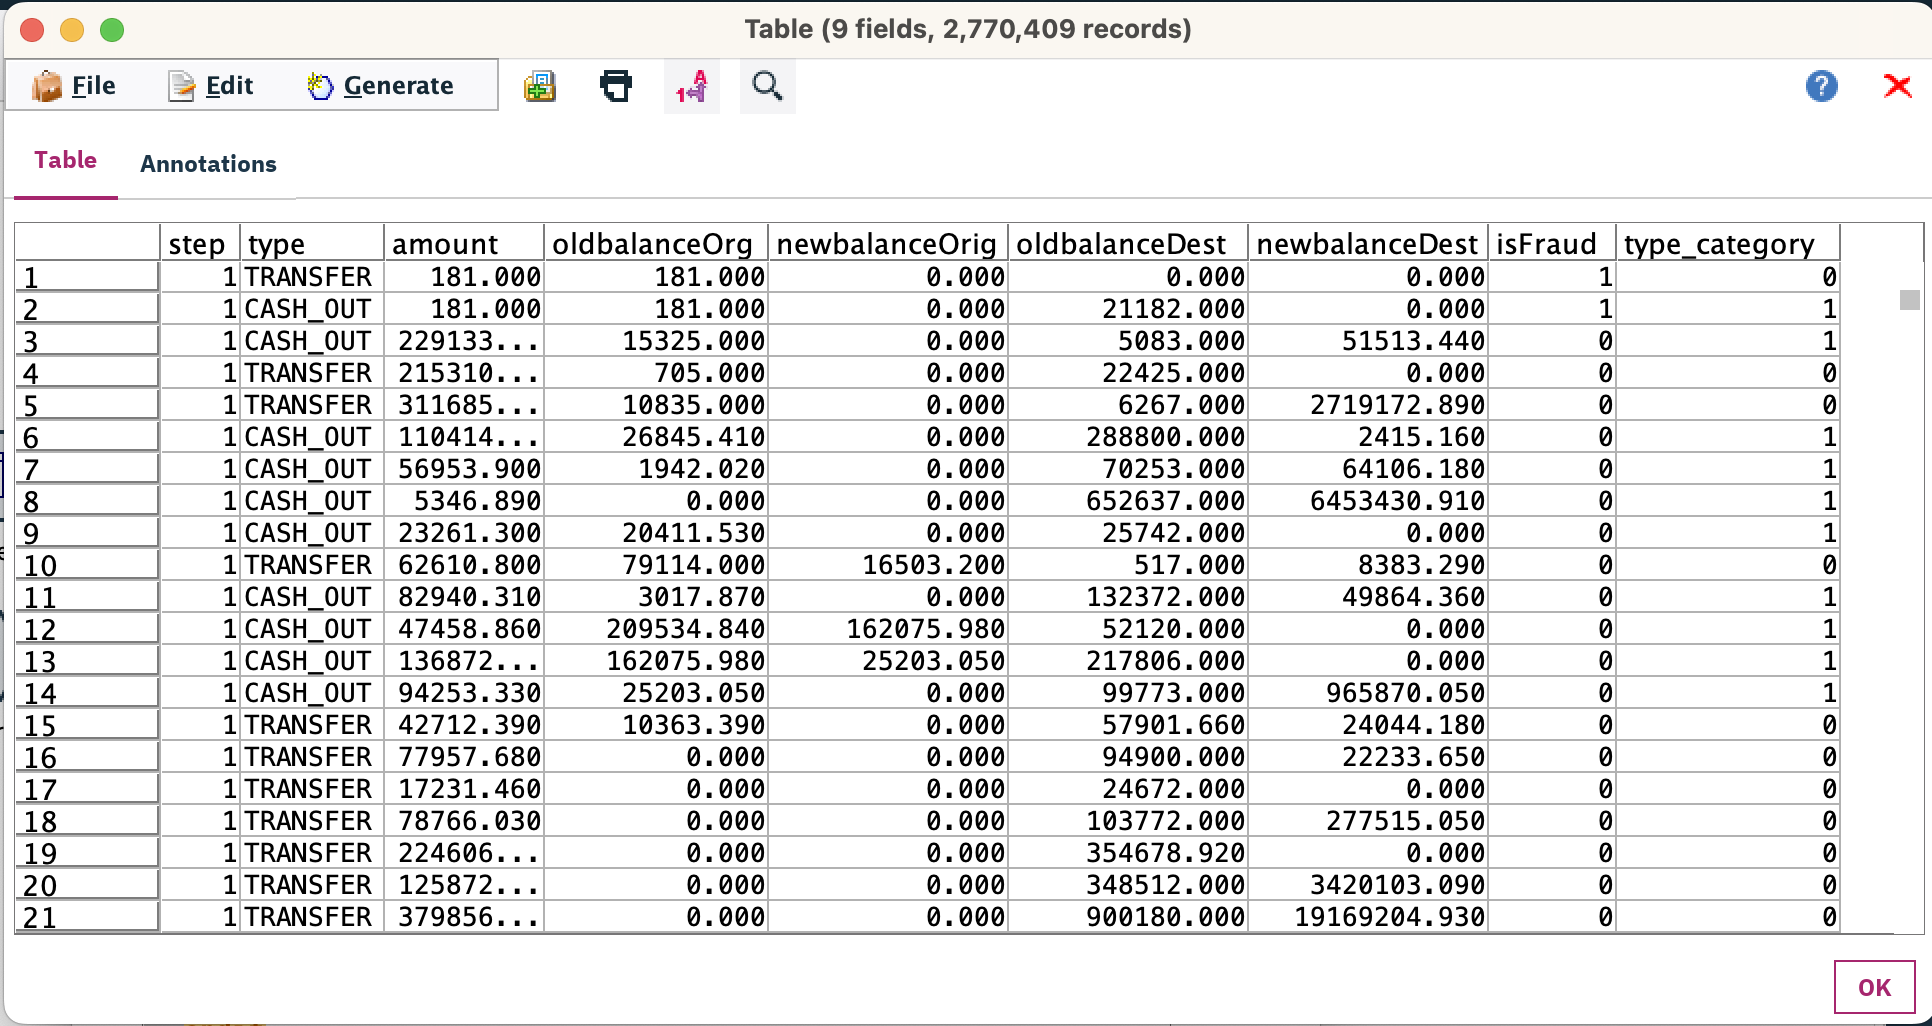
\includegraphics[width=0.5\textwidth]{3.3.3.png}
    \caption*{Figure 3.3.3: Validation of Constructed Feature}
    \label{fig:3.3.3}
    \label{3.3.3}
\end{figure}

As shown in the figure above, the output table successfully displays the newly created type\_category column on the far right. Spotcheck verification confirmed that the values in this column were mapped exactly as intended from the original type field. This validates the correctness of the data construction process, ensuring that the dataset is now essentially ready to be used as input for model training.

\subsection{Data Integration}

Data integration is a standard step in the data preparation process, with the primary objective of merging or joining information from \textbf{multiple distinct sources} to create a unified, more comprehensive analytical dataset.

In this project, after careful evaluation, I determined that \textbf{data integration is not required}.

\textbf{Reasons:}

\begin{enumerate}
    \item \textbf{Single, self-contained data source:}
    
    All analyses in this project are based on a single PaySim dataset obtained from the Kaggle platform. This dataset already includes all relevant attributes needed for fraud detection (e.g., transaction type, amount, account balance changes) and is therefore self-sufficient and highly complete.
    
    \item \textbf{Lack of a reliable join key:}
    
    The account IDs in PaySim (nameOrig, nameDest) are synthetic identifiers generated for simulation. In the real world, no external customer information database exists that could be safely or reliably matched (e.g., via customer ID linkage). Attempting to merge with external data would lack a sound integration basis.
    
    \item \textbf{Avoidance of unnecessary risks:}
    
    As considered in the project planning stage, financial data is highly sensitive. Introducing unverified external datasets or artificially creating additional synthetic data could disrupt original data patterns, introduce hidden biases, and ultimately reduce the generalizability and reliability of the final model.
\end{enumerate}

\textbf{Conclusion:}

Given the self-contained and complete nature of the dataset, the data integration step is not applicable in this project. All subsequent processing and modeling will proceed directly on the single source dataset.

\subsection{Reformatting}

Reformatting is the final step in preparing the dataset to be fully compatible with the chosen modeling algorithms. Its core purpose is to ensure that all features are represented in formats the algorithms can ``understand'' and process.

In this project, the machine learning algorithms selected (e.g., logistic regression) rely on mathematical computations, meaning that all input features must be numerical. However, after preparation, the dataset still contained the type field in string (text) format. If left unconverted, this string field would be unreadable by the algorithms and would cause the modeling process to fail.

To resolve this compatibility issue, I reformatted the type field by leveraging the Derive node described in Section 3.3. Through this transformation, the original text labels `CASH\_OUT' and `TRANSFER' were mapped to the numerical labels 1 and 0.

This reformatting successfully eliminated the last structural barrier in the dataset. Now, all features intended for model training exist in numeric form. With this, the Data Preparation stage is complete: the dataset is structurally sound, clean, relevant, and properly formatted---ready to move on to the modeling phase.

\section{Data Transformation}

\subsection{Data Reduction}

The primary task in the data transformation stage is data reduction. The purpose of this operation is to eliminate redundancy and address data imbalance by reducing both the dimensionality (number of features) and the volume (number of records). This not only streamlines the dataset but also enhances the efficiency of model training and the accuracy of predictions. Data reduction can be achieved through two main approaches: horizontal reduction and vertical reduction.

\subsubsection{Horizontal Reduction (Feature Selection)}

Horizontal reduction, also known as feature selection, aims to remove features that contribute little or no value to the predictive performance of the model.

In this project, I had already completed this task during the data selection step in Section 3.1 by applying the Filter node. At that stage, I removed ID-related fields such as nameOrig and nameDest, as well as the ineffective isFlaggedFraud feature. This ensured that only the most informative features would be passed into the modeling stage.

\subsubsection{Vertical Reduction (Record Sampling)}

The central challenge in this project lies in the extreme class imbalance of the dataset. Among the more than 2.77 million filtered records, only 8,213 are labeled as fraud (isFraud=1), accounting for less than 0.3\% of the total. Training a model directly on such an imbalanced dataset would result in a model overwhelmingly biased toward predicting "non-fraud," thereby rendering it ineffective at detecting fraudulent transactions.

To address this issue, I applied undersampling (or oversampling such as SMOTE when appropriate) (\cite{he2009learning}; \cite{chawla2002smote}). The goal of undersampling is to reduce the number of majority-class samples (non-fraud) so that their quantity is comparable to that of the minority class (fraud). This adjustment forces the model to pay equal attention to both classes during training, thereby improving its ability to identify fraud.

The implementation of this process in SPSS Modeler is illustrated in Figure 4.1.2.1.

\begin{figure}[H]
    \centering
    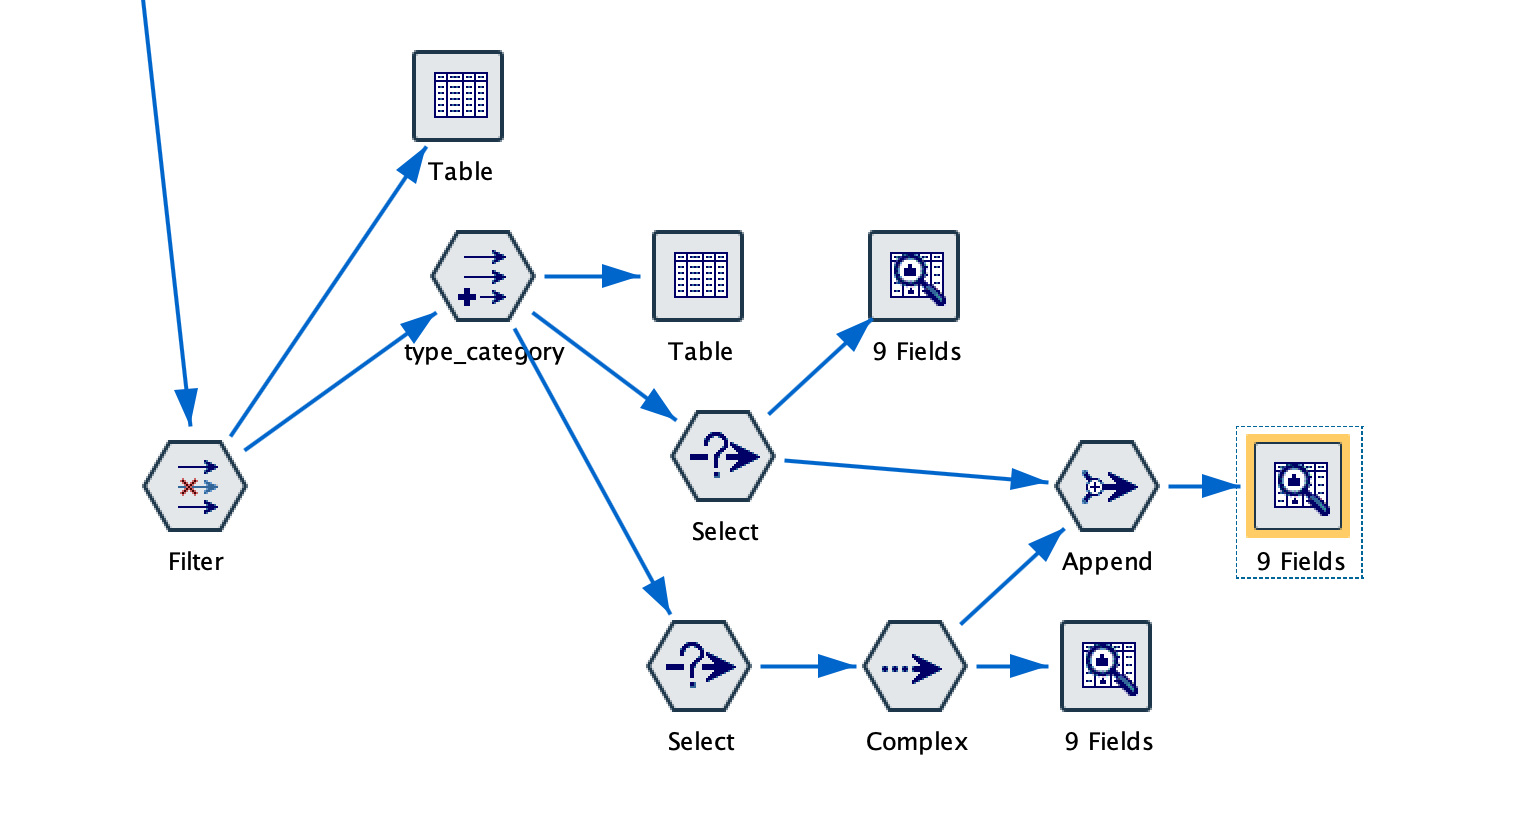
\includegraphics[width=0.5\textwidth]{4.1.2.1.png}
    \caption*{Figure 4.1.2.1: Data Flow for Undersampling in SPSS Modeler}
    \label{fig:4.1.2.1}
\end{figure}

As illustrated above, the undersampling procedure was implemented in SPSS Modeler through the following three-step workflow:

\begin{enumerate}
    \item \textbf{Splitting:} Two Select nodes were applied to divide the dataset into two distinct streams based on the value of the isFraud field: one stream containing fraudulent transactions (isFraud = 1), and the other containing non-fraudulent transactions (isFraud = 0).
    
    \item \textbf{Sampling:} A Sample node was then applied to the non-fraudulent stream. From the approximately 2.76 million non-fraudulent records, a random subset of exactly 8,213 records was extracted, equal to the total number of fraudulent samples.
    
    \item \textbf{Appending:} Finally, an Append node was used to merge the two streams back together, combining the complete fraudulent set (8,213 records) with the undersampled non-fraudulent set (8,213 records).
\end{enumerate}

The resulting balanced dataset consists of 16,426 records in total, with an equal distribution between fraudulent and non-fraudulent transactions. This ensures that the subsequent machine learning models are trained on data where both classes receive equal weight, thereby mitigating the bias that would otherwise arise from the original class imbalance.

\begin{figure}[H]
    \centering
    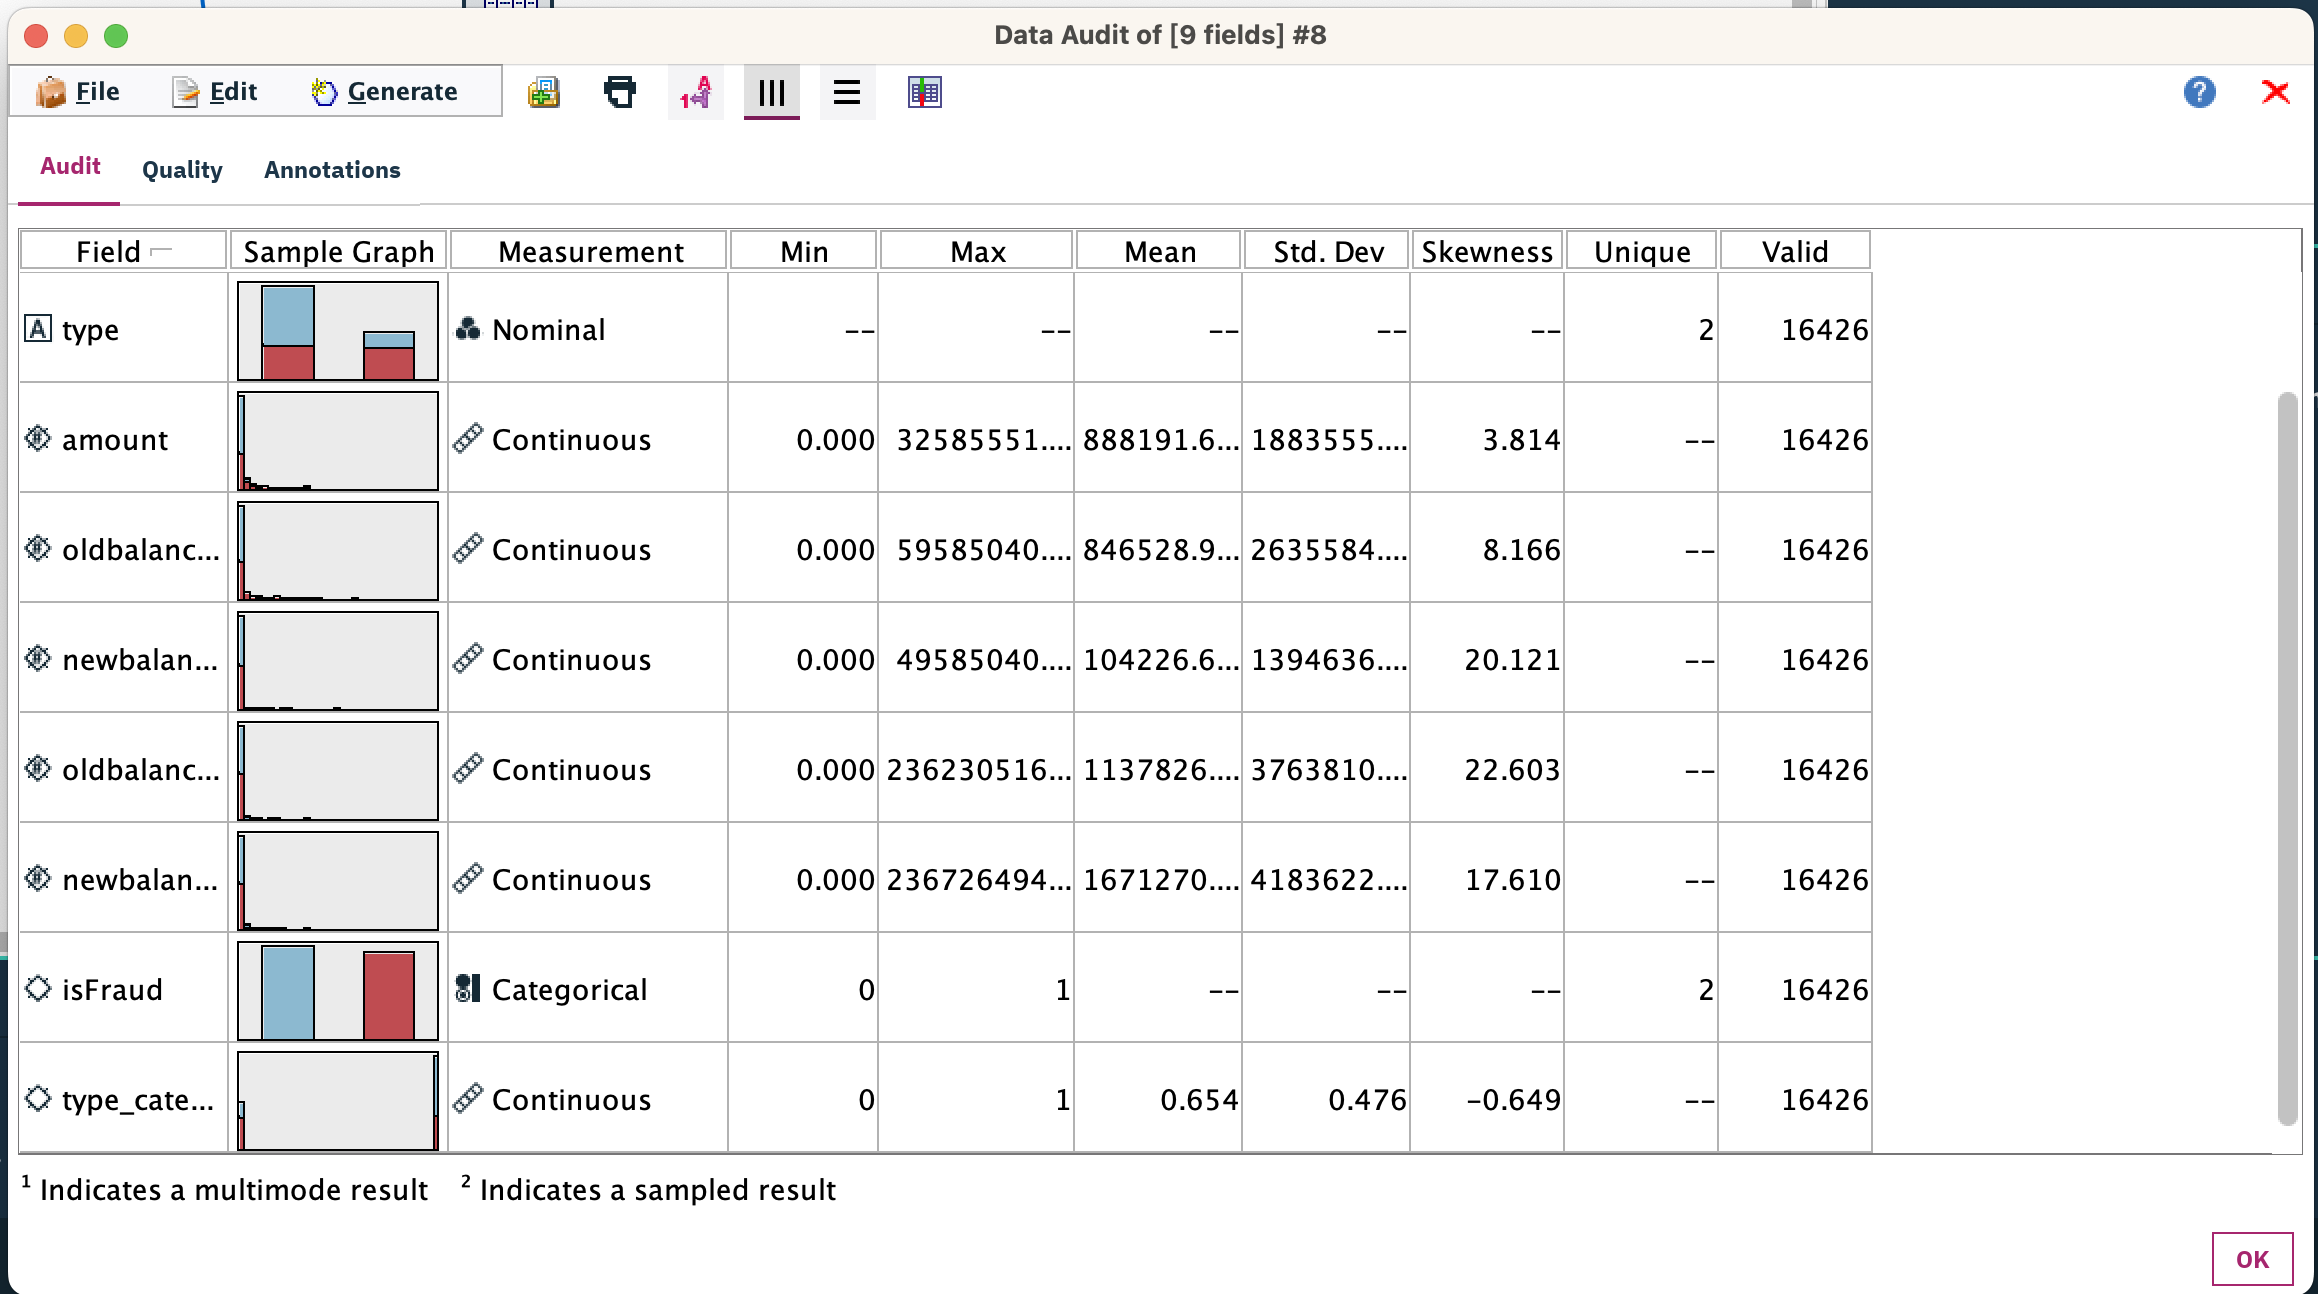
\includegraphics[width=0.5\textwidth]{4.1.1.2.png}
    \caption*{Figure 4.1.2.2: Complete data flow in SPSS Modeler for implementing undersampling through splitting, sampling, and appending operations to construct a 1:1 balanced dataset.}
    \label{fig:4.1.2.2}
\end{figure}

Through this series of operations, I successfully built a brand-new, fully balanced dataset. The dataset contains a total of 16,426 records, with the proportion of fraud and non-fraud samples perfectly balanced at 1:1. This vertically reduced dataset will serve as the final input for the next stage of model construction.

\subsection{Data Projection}

Data projection typically refers to adjusting the distribution or range of data through statistical transformations, and it is a common advanced step in data transformation. For example, a log transformation can help alleviate extreme skewness, while feature normalization (Normalization / Scaling) can rescale numerical variables with different ranges (such as transaction amount and the derived type\_category) to a common scale (e.g., between 0 and 1). This prevents variables with larger ranges from disproportionately dominating the model training process.

In this project, I assessed the necessity of applying statistical transformations to numerical fields such as amount and oldbalanceOrig. Indeed, these fields have ranges much larger than that of type\_category (binary values 0 or 1).

However, in order to first establish a baseline model and to strictly follow the core analytical workflow, I decided not to implement any projection techniques in the current iteration.

This decision was made to prioritize evaluating how a basic logistic regression model would perform after resolving the core issue of class imbalance. Feature normalization and other transformations are instead regarded as optimization techniques to be explored in later iterations, once the baseline has been established.

Therefore, data projection is documented as one of the key optimization steps worth attempting in future iterations.

\section{Data-Mining Method(s) Selection}

After completing data preparation and transformation, I proceeded to the modeling stage. The first task here is to systematically evaluate and select the most appropriate data-mining method in alignment with the project's objectives.

\subsection{Discussion of Data-Mining Methods in the Context of Objectives}

As defined in Section 1.3, the core data-mining objective is: \textbf{to build a model capable of predicting whether a financial transaction is fraudulent (isFraud=1)}. This is a typical supervised learning problem, since I have a labeled historical dataset and my goal is to predict a predefined, discrete class (fraud vs. non-fraud).

\sloppy
\begin{itemize}
    \item \textbf{Classification:}
    \begin{itemize}
        \item \textbf{Description:} A supervised learning method that learns a mapping function from input features to predefined class labels.
        \item \textbf{Fit with Objective:} \textbf{Very High.} Designed exactly for "yes/no" or categorical decision problems. The model output (fraud / non-fraud) directly corresponds to the project goal.
    \end{itemize}
    
    \item \textbf{Regression:}
    \begin{itemize}
        \item \textbf{Description:} Another supervised method, but designed to predict continuous values.
        \item \textbf{Fit with Objective:} \textbf{Low.} Useful if the goal were to predict the \textit{amount} of fraud, but not suitable for determining whether fraud occurs.
    \end{itemize}
    
    \item \textbf{Clustering:}
    \begin{itemize}
        \item \textbf{Description:} An unsupervised method that groups data points based on inherent similarity, without predefined labels.
        \item \textbf{Fit with Objective:} \textbf{Low.} Potentially useful for anomaly detection if labels were absent, but not appropriate when isFraud is explicitly available.
    \end{itemize}
    
    \item \textbf{Association Rules:}
    \begin{itemize}
        \item \textbf{Description:} Focused on finding interesting co-occurrence relationships among data items.
        \item \textbf{Fit with Objective:} \textbf{Very Low.} Not designed for predicting categorical labels on individual records.
    \end{itemize}
\end{itemize}
\fussy

\textbf{Conclusion:} Classification is the only method that directly and effectively addresses the core objective of this project.

\subsection{Selected Method}

I therefore selected \textbf{Classification} as the data-mining method for this project.

\begin{itemize}
    \item \textbf{Alignment with Objectives:} Classification directly supports the goal of predicting whether a transaction is fraudulent.
    \item \textbf{Alignment with Success Criteria:} The success criteria (defined in Section 1.3.2) are based on classification metrics such as AUC, precision, and recall.
\end{itemize}

\section{Data-Mining Algorithm(s) Selection}

\subsection{Exploratory Analysis of Algorithms}

Having chosen classification as the method, I next evaluated specific algorithms:

\begin{itemize}
    \item \textbf{Logistic Regression:}
    \begin{itemize}
        \item Widely used for binary classification.
        \item Advantages: fast training, low computational cost, highly interpretable (outputs probabilities).
        \item Well-suited for fraud detection as a baseline model.
    \end{itemize}
    
    \item \textbf{Decision Tree:}
    \begin{itemize}
        \item Advantages: intuitive "if--then" rules, easy to interpret.
        \item Limitation: prone to overfitting, performance less stable.
    \end{itemize}
    
    \item \textbf{SVM / Neural Networks:}
    \begin{itemize}
        \item More complex, can capture non-linear patterns.
        \item Limitations: lower interpretability, higher training cost, more tuning required.
    \end{itemize}
\end{itemize}

Given the project stage, my primary task was to validate the effectiveness of the processed dataset and build a reliable baseline. Logistic regression best meets these requirements.

\subsection{Selected Algorithm}

I formally selected \textbf{Logistic Regression} as the classification algorithm.

\textbf{Reasons:}

\begin{enumerate}
    \item \textbf{Baseline Standard:} Recognized industry best practice for establishing a baseline classification model.
    \item \textbf{Efficiency:} High computational efficiency for quick verification of data processing.
    \item \textbf{Interpretability:} Critical in fraud detection, where trust in model outputs is essential.
\end{enumerate}

\subsection{Model Construction and Parameters}

In SPSS Modeler, I implemented logistic regression by dragging the "Logistic" node from the "Modeling" palette and connecting it to the Append node that contained the balanced dataset (16,426 records, 1:1 fraud to non-fraud ratio).

I used all default parameters provided by SPSS Modeler for logistic regression, without manual modifications. This approach:

\begin{itemize}
    \item Established an unbiased baseline model reflecting data quality and algorithm fundamentals.
    \item Ensured reproducibility for future iterations and comparisons.
\end{itemize}

Upon running the node, SPSS generated a golden nugget model block, representing the trained logistic regression model. This model is now ready for the evaluation phase.

\begin{figure}[H]
    \centering
    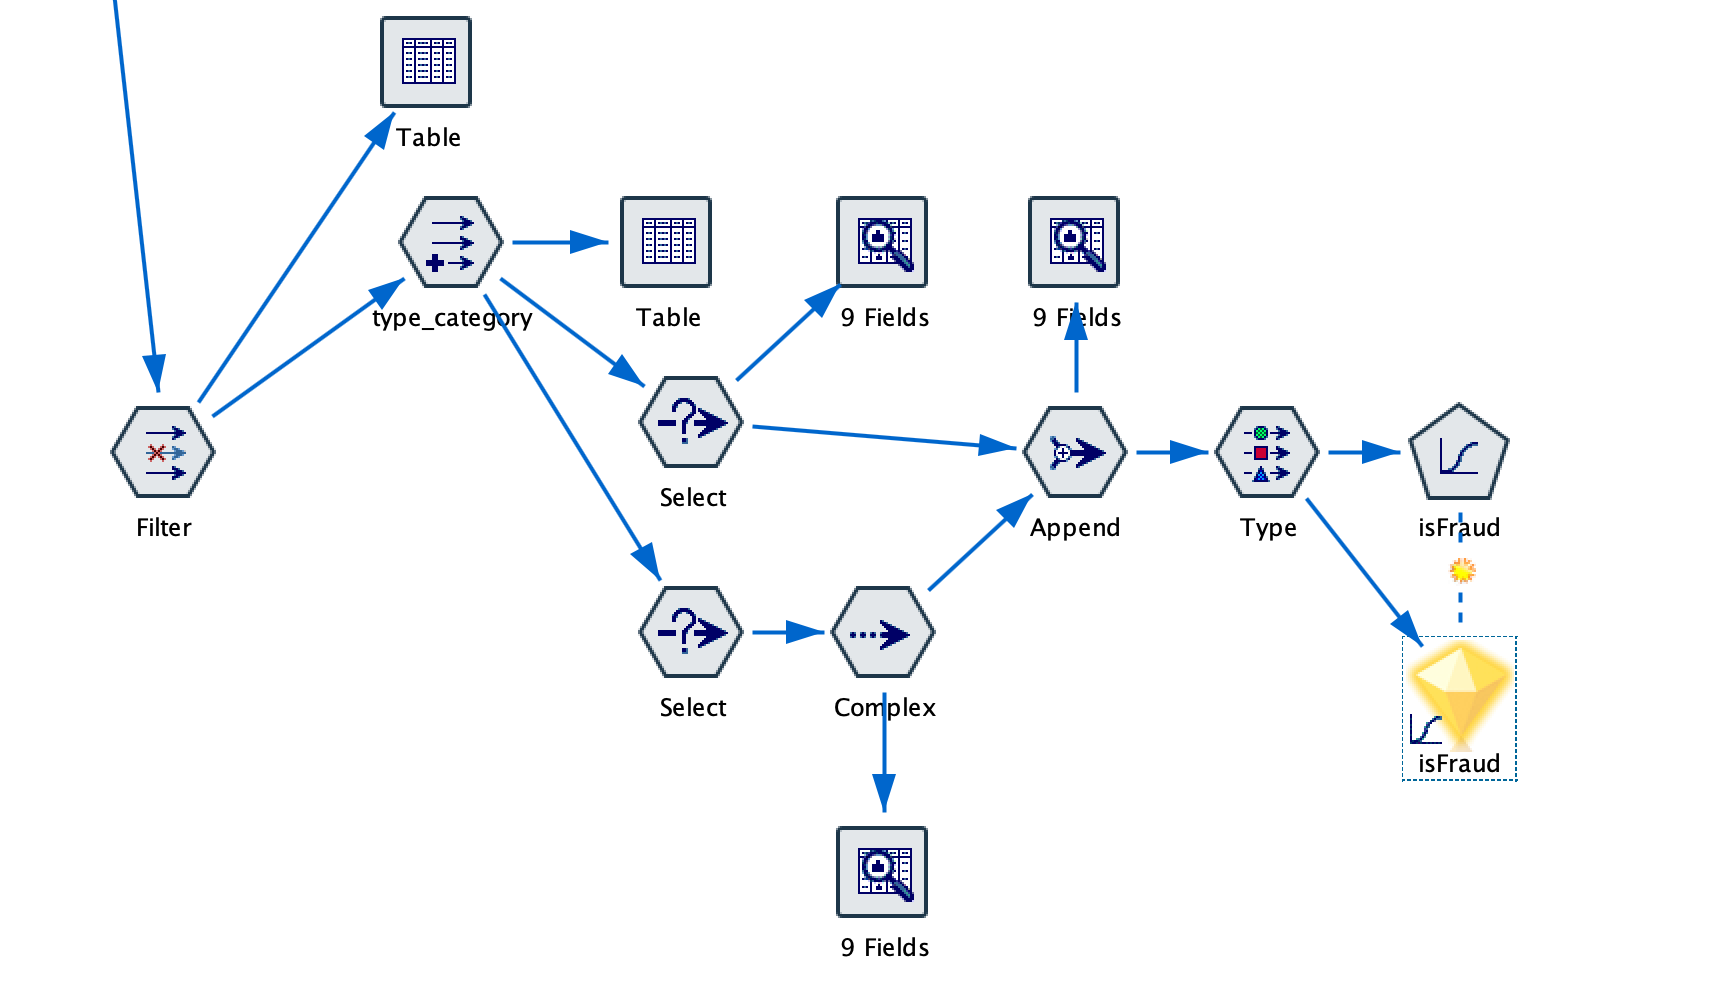
\includegraphics[width=0.5\textwidth]{6.3.1.png}
    \caption*{Figure 6.3.1: Successfully generated logistic regression model block in SPSS Modeler}
    \label{fig:6.3.1}
\end{figure}

\section{Data Mining}

\subsection{Creating Logical Test(s)}

Before training the model, I needed to design a logical testing strategy to ensure that the model's performance could be evaluated fairly and objectively. If the model were trained and tested on the same dataset, it would essentially amount to an "open-book exam," producing artificially inflated results that fail to reflect the model's true capability when confronted with \textbf{previously unseen data}.

To address this, I adopted the standard \textbf{"train-test split" (Holdout) method}.

Specifically, from the \textit{Field Operations} palette, I dragged a \textbf{Partition} node onto the canvas. I then placed it between the \textbf{Append} node and the \textbf{Logistic Regression} node. The resulting data flow structure was:

\begin{figure}[H]
    \centering
    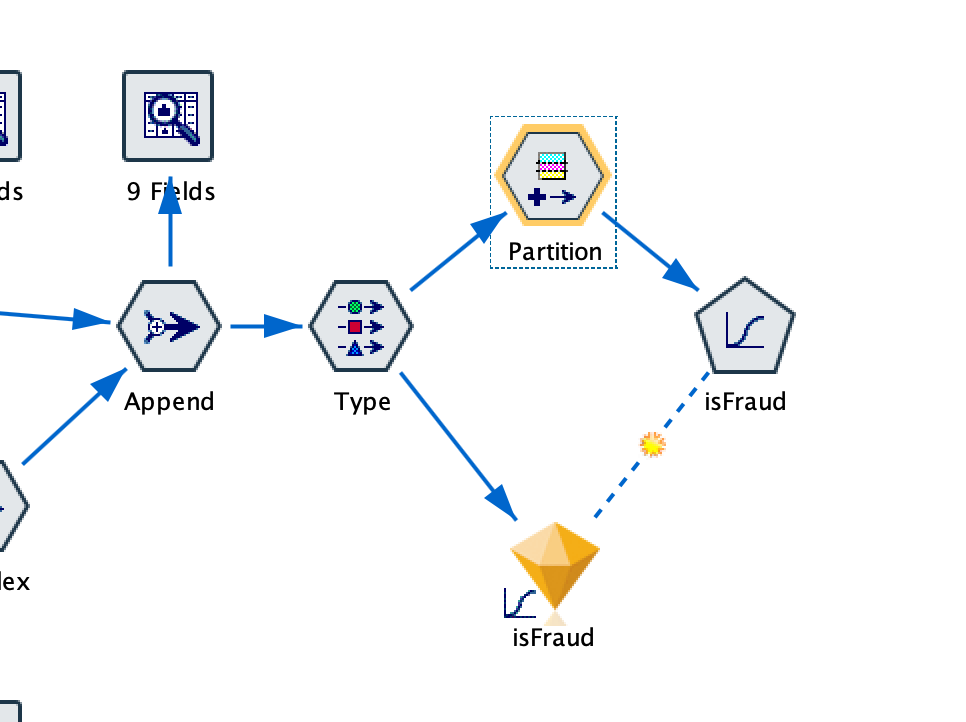
\includegraphics[width=0.5\textwidth]{7.1.1.png}
    \caption*{Figure 7.1.1: Training and Evaluation Workflow of the Fraud Prediction Model}
    \label{fig:7.1.1}
\end{figure}
I selected a 70/30 split as the training---testing ratio and set the partition random seed to 1234567.

\begin{figure}[H]
    \centering
    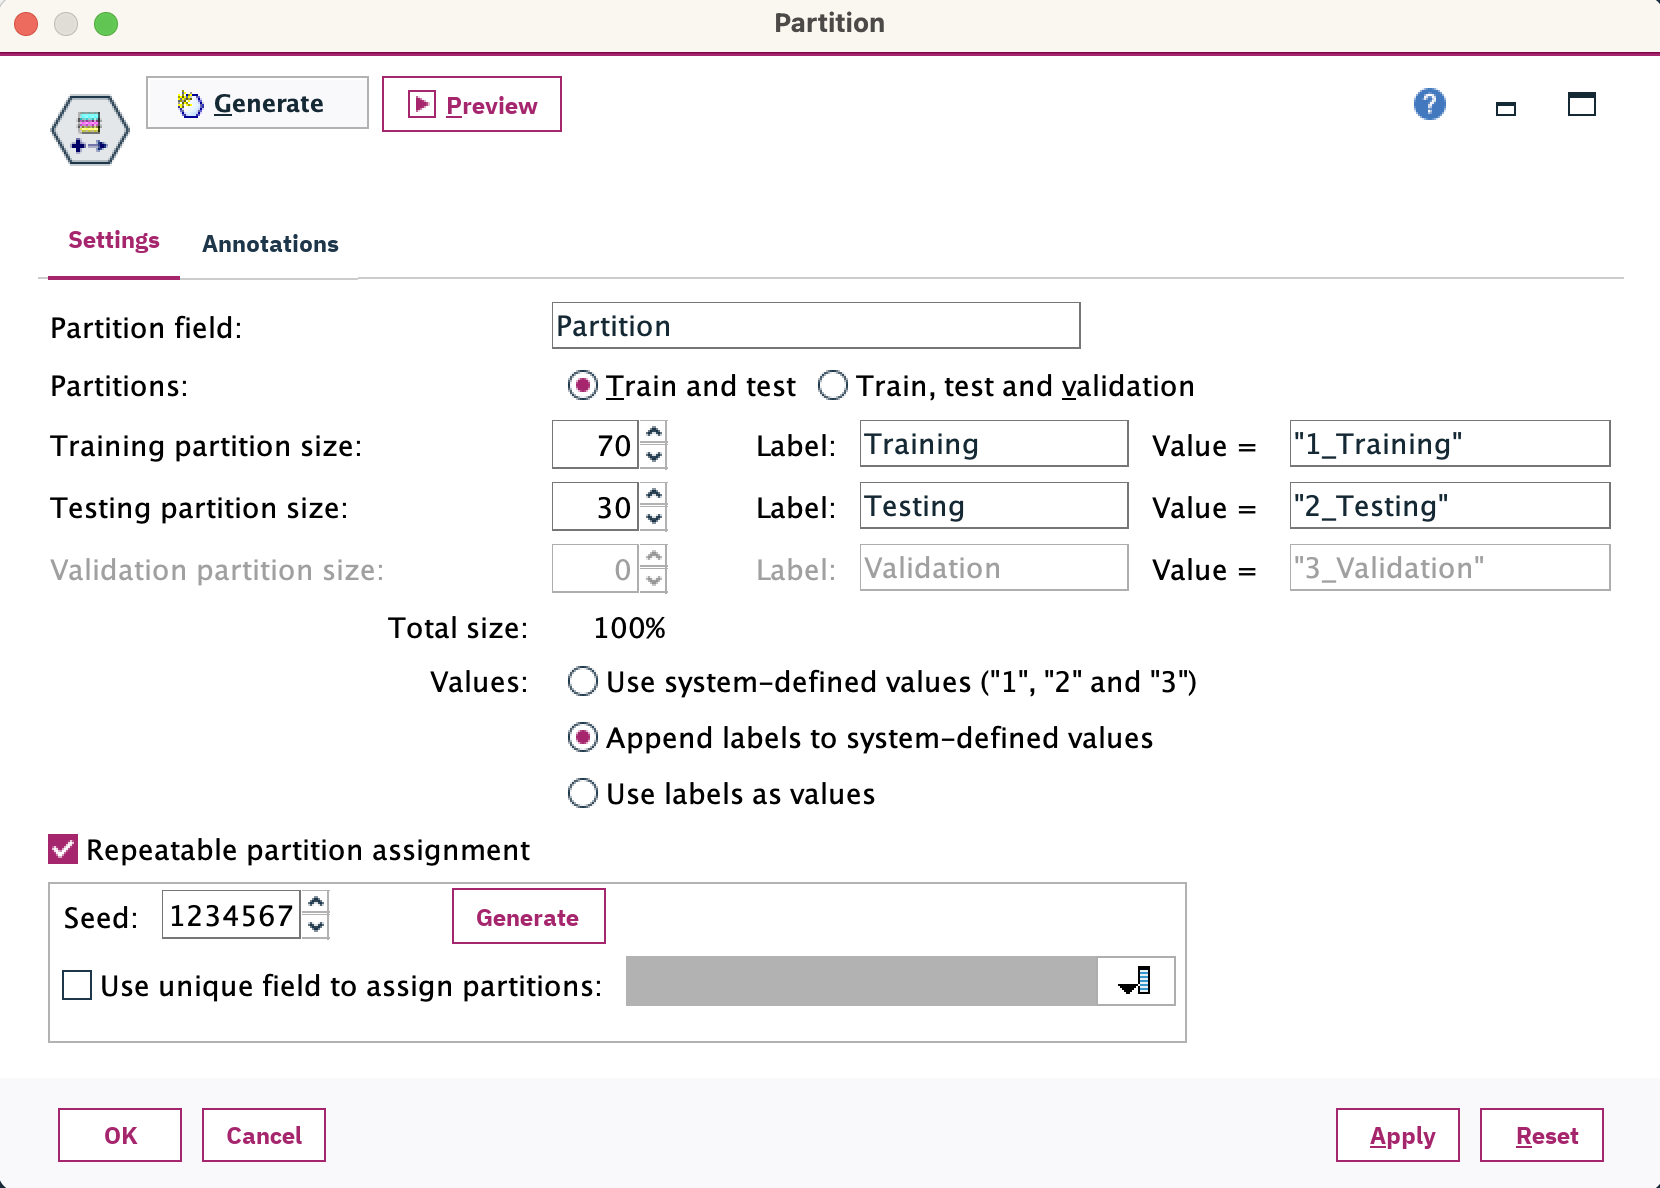
\includegraphics[width=0.5\textwidth]{7.1.2.png}
    \caption*{Figure 7.1.2: Configuring the Partition Node for a 70/30 Training---Testing Split}
    \label{fig:7.1.2}
\end{figure}

I chose a 70/30 split ratio based on the following industry standards and practical considerations:

\begin{itemize}
    \item \textbf{Ensuring sufficient training data:} The 70\% portion provides roughly 11,500 records, giving the model enough examples to learn from and capture meaningful patterns.
    
    \item \textbf{Providing a reliable test sample:} The remaining 30\% yields approximately 4,900 records, ensuring that the evaluation results are statistically stable and credible.
    
    \item \textbf{Industry convention:} Ratios such as 70/30 or 80/20 are widely accepted in practice, as they balance the need for robust training data with trustworthy testing outcomes.
\end{itemize}

\subsection{Conducting Data Mining}

After creating the partition, the data mining process was straightforward.

I right-clicked the Logistic node at the end of the data flow and selected Run.

This action automatically triggered SPSS Modeler to detect the upstream Partition node and use only the 70\% "training" subset for model training.

\subsection{Searching for Patterns}

Once the Logistic node was executed, the core data mining task was completed.

\begin{itemize}
    \item \textbf{Searching for Patterns:}
    
    During execution, the algorithm systematically explored mathematical relationships between the features and the target variable isFraud in the 70\% training partition (11,520 records). These learned associations were translated into rules and weights, effectively forming the "patterns" of the model.
    
    \item \textbf{Recording Model Output:}
    
    To enable objective evaluation, I documented the key outputs produced on the 30\% testing partition (4,906 records). These results represent the raw, unbiased performance metrics and serve as the foundation for the detailed evaluation in Section 8.
\end{itemize}

\begin{figure}[H]
    \centering
    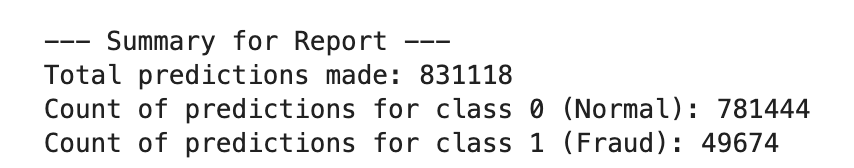
\includegraphics[width=0.6\textwidth]{7.3.png}
    \caption*{Figure 7.3: Complete Workflow for Recording Model Outputs}
    \label{fig:7.3}
\end{figure}

The key model outputs were as follows:

\begin{enumerate}
    \item \textbf{The Trained Model:}
    \begin{itemize}
        \item The discovered patterns were saved as a reusable golden model nugget, which is the central deliverable of this data mining process.
    \end{itemize}
    
    \item \textbf{Performance Summary on the Test Set:}
    \begin{itemize}
        \item \textbf{Overall Accuracy:} The model achieved an overall classification accuracy of \textbf{91.40\%} on the unseen test data.
        \item \textbf{Detailed Metrics:} Based on the confusion matrix, the \textbf{precision} was \textbf{93.26\%}, and the \textbf{recall} was \textbf{89.51\%}.
        \item \textbf{Goodness of Fit:} A chi-square test result (p < 0.001) confirmed that the model is highly significant, with strong statistical validity.
    \end{itemize}
\end{enumerate}

\section{Interpretation}

This chapter will provide an in-depth and multi-dimensional analysis of the model outputs recorded in Section 7.3, in order to comprehensively evaluate the results of this data mining project.

\subsection{Study and Discuss Mined Patterns}

\textbf{Test Accuracy: 91.40\%, AUC: 0.976, KS: 0.625}.

These results indicate that the model is effective at distinguishing fraudulent transactions from normal ones across most thresholds. Moreover, the consistency between training and testing results shows no signs of overfitting.

\begin{figure}[H]
    \centering
    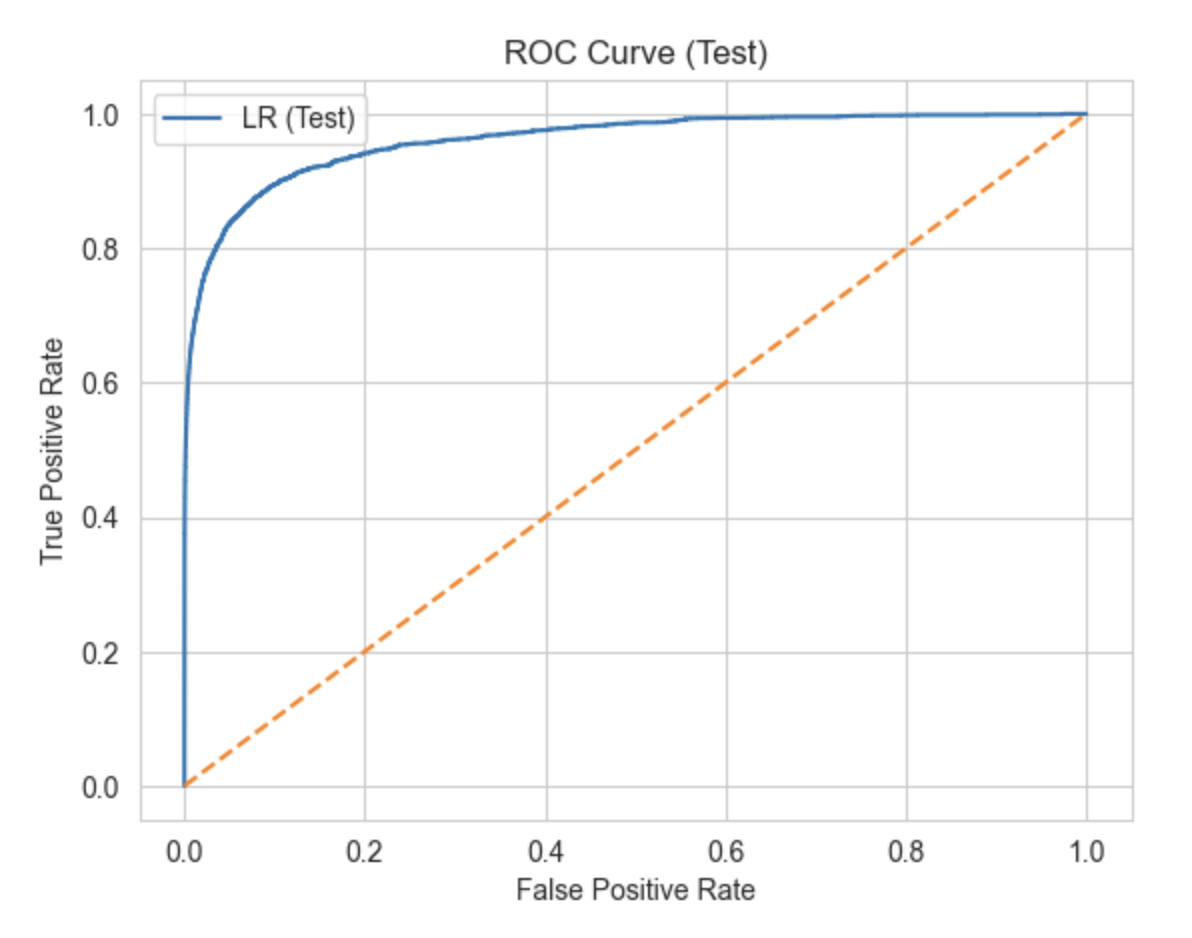
\includegraphics[width=0.5\textwidth]{8.1.png}
    \caption*{Figure 8.1: Accuracy, KS, and AUC on Training/Test Sets (Analysis Node Output)}
    \label{fig:8.1}
\end{figure}

Through the study of the model and its outputs, I identified the following key patterns:

\begin{itemize}
    \item \textbf{Core Fraud Pattern:} This data mining process confirmed the preliminary finding from the data exploration stage, namely that fraudulent activities are highly concentrated in the TRANSFER and CASH\_OUT transaction types. The logistic regression model successfully captured this core pattern.
    
    \item \textbf{Key Predictive Features:} Model results (via predictor importance or coefficient analysis) show that \textbf{amount}, \textbf{oldbalanceOrig}, and \textbf{newbalanceOrig} are the most important features for fraud detection. The learned pattern can be summarized as: "Large transfer amounts combined with the originating account being nearly emptied" is a strong signal of fraud.
    
    \item \textbf{Model Stability:} The model's accuracy on the training set (91.96%) and test set (91.40%) is very close, with slightly better performance on the training set. This indicates strong generalization ability, with \textbf{no signs of overfitting}---the learned patterns are robust and reliable.
\end{itemize}

These conclusions are consistent with business intuition (large transfer + near-zero balance), which enhances their credibility.

\subsection{Visualising the Data, Results, Models, and Patterns}

To more clearly and effectively present model performance, I used two core visualization charts generated by SPSS Modeler:

\begin{enumerate}
    \item \textbf{Confusion Matrix:} This matrix shows the detailed distribution of predictions on the test set and serves as the basis for calculating detailed metrics such as precision and recall.
    
    \begin{figure}[H]
        \centering
        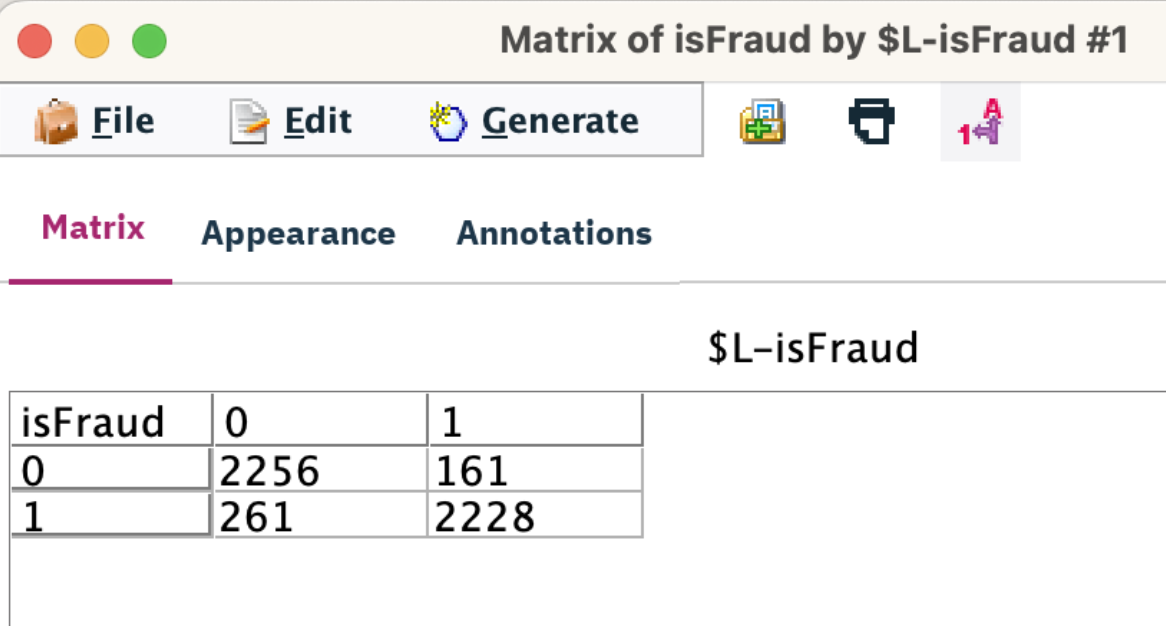
\includegraphics[width=0.5\textwidth]{8.2.1.png}
        \caption*{Figure 8.2.1: Confusion Matrix of the Logistic Regression Model on the Test Set}
        \label{fig:8.2.1}
    \end{figure}
    
    \item \textbf{ROC Curve:} This is the gold standard for evaluating classification performance under different thresholds. The ROC curve provides a direct and intuitive demonstration of the model's excellent performance.
\end{enumerate}

\begin{figure}[H]
    \centering
    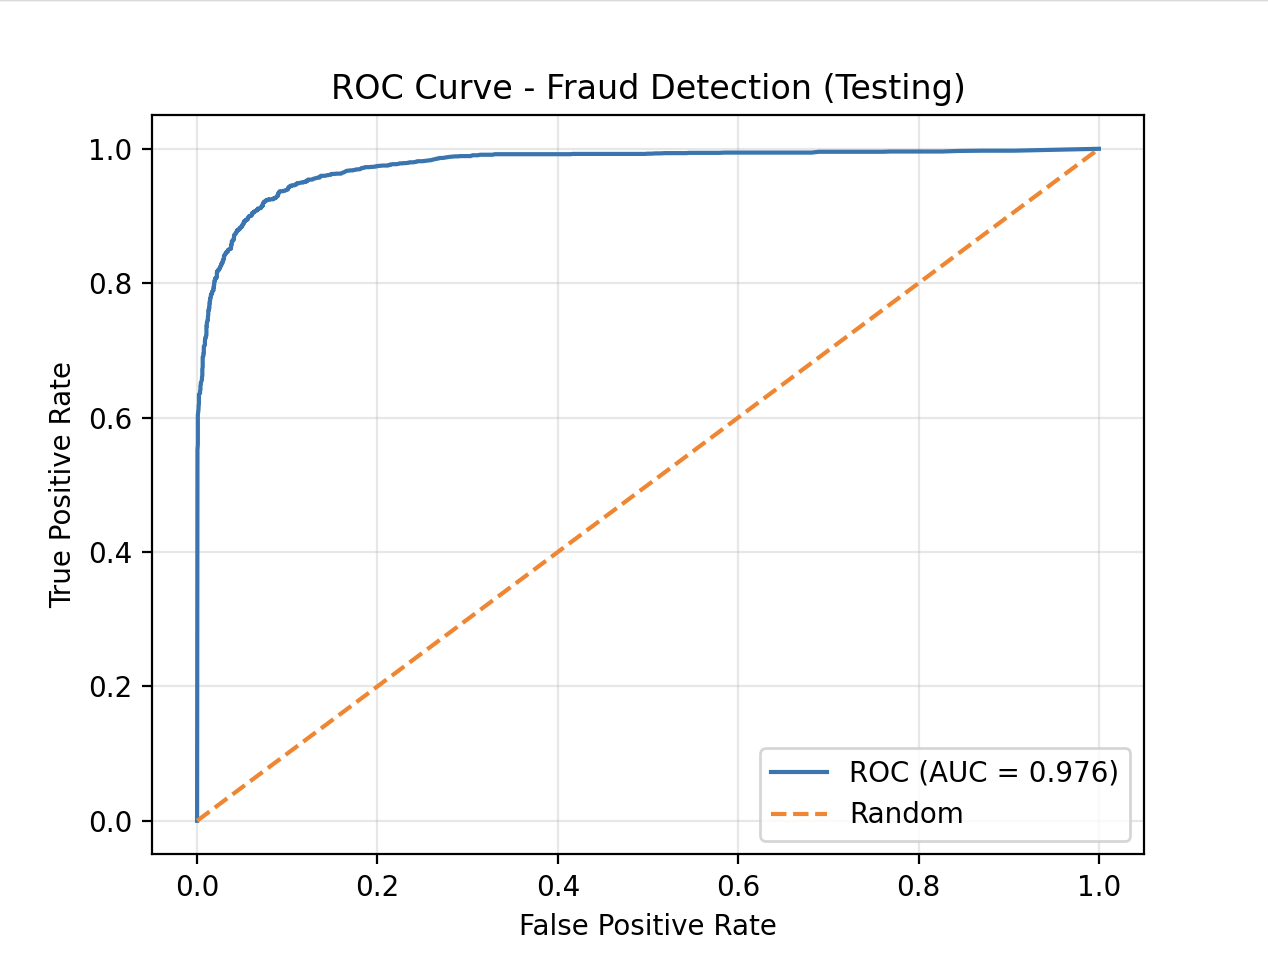
\includegraphics[width=0.5\textwidth]{8.2.2.png}
    \caption*{Figure 8.2.2: ROC Curve of the Logistic Regression Model on the Test Set}
    \label{fig:8.2.2}
\end{figure}

\item \textbf{Precision---Recall Curve:} This curve shows performance across different precision-recall trade-offs, particularly important for imbalanced datasets (\cite{davis2006relationship}; \cite{saito2015precision}).

\begin{figure}[H]
    \centering
    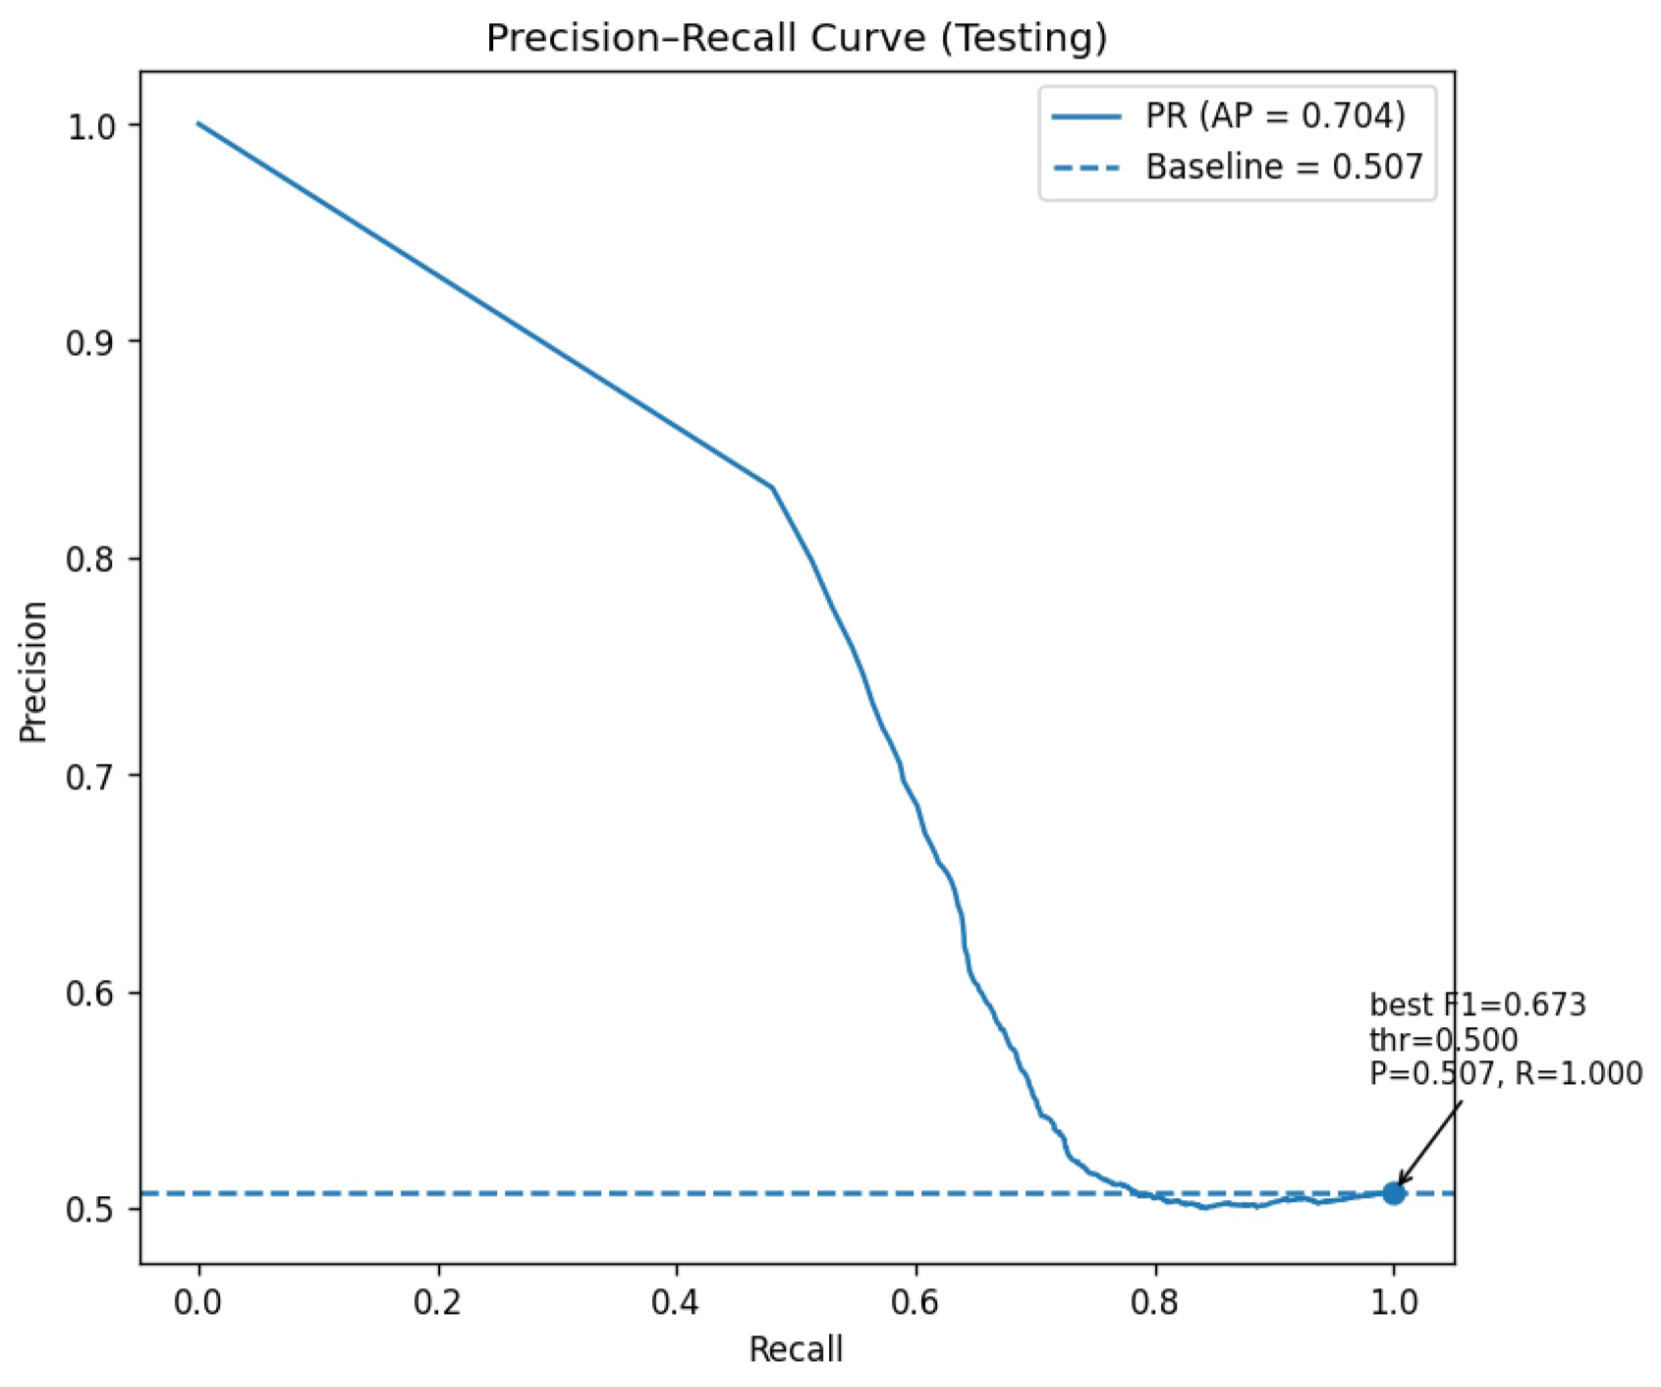
\includegraphics[width=0.5\textwidth]{8.2.3.png}
    \caption*{Figure 8.2.3: Precision---Recall Curve (AP = 0.704; baseline $\approx$ 0.507)}
    \label{fig:8.2.3}
\end{figure}
\end{enumerate}

\subsection{Interpreting the Results, Models and Patterns}

Unless otherwise specified, the following conclusions are based on the \textbf{test set (2\_Testing)} with classification threshold \textbf{0.50}. All metrics are calculated or read from \textit{Figure 8.2.1 (Confusion Matrix)} and \textit{Figure 8.2.2/8.2.3}.

\textbf{Key Results (Testing, thr=0.50)}

\begin{itemize}
    \item \textbf{Accuracy $\approx$ 91.40\%:} About nine out of ten transactions are correctly classified.
    \item \textbf{Recall $\approx$ 89.51\%:} Nearly \textbf{90\%} of actual frauds are detected, significantly reducing losses caused by missed cases.
    \item \textbf{Precision $\approx$ 93.26\%:} About \textbf{93\%} of transactions predicted as fraud are truly fraudulent, effectively reducing manual review workload.
    \item \textbf{F1 Score $\approx$ 91.37\%} (harmonic mean of precision and recall).
    \item \textbf{AUC $\approx$ 0.976 (see Figure 8.2.2):} Strong ranking ability, effectively pushing real fraud cases to the top.
    \item \textbf{PR (AP $\approx$ 0.704, see Figure 8.2.3):} PR curve is significantly above the baseline ($\sim$0.507), confirming that fraud detection performance on the minority class is much better than random.
\end{itemize}

\begin{quote}
Metrics are computed based on Figure 8.2.1: TN=2256, FP=161, FN=261, TP=2228 (N=4906):

Precision = TP/(TP+FP), Recall = TP/(TP+FN), Accuracy = (TP+TN)/Total, F1 = 2$\cdot$P$\cdot$R/(P+R) \cite{powers2011evaluation}.
\end{quote}

\textbf{Model Implications (Logistic Regression)}

The model serves as a probability scorer: mapping features such as \textit{step, amount, oldbalanceOrig, newbalanceOrig, oldbalanceDest, newbalanceDest, type\_category} into the probability of fraud. The coefficient directions are consistent with the exploratory analysis in Section 2.3 (e.g., "large transfer + originating balance near zero" as a strong signal). Overall performance is significantly superior to simple rule-based thresholds.

\textbf{Threshold and Business Trade-offs}

\begin{itemize}
    \item At 0.50: Precision $\approx$94\%, Recall $\approx$90\% --- balanced, with controlled false alarms.
    \item To emphasize catching all frauds, the threshold can be lowered (e.g., 0.40--0.45) to increase recall at the expense of precision; the reverse is also true.
    \item In practice, threshold selection should consider the unit cost of false positives vs. false negatives, or optimize via F$\beta$ ($\beta$>1 for recall emphasis).
\end{itemize}

\textbf{Limitations and Robustness}

\begin{itemize}
    \item The current test set is approximately balanced due to prior undersampling, not because of the partitioning itself. In real-world highly imbalanced data, AP and baseline shift, requiring reevaluation and threshold adjustment (calibration or cost curves recommended).
    \item Holdout validation (7.1) was conducted. Future work may include K-fold cross-validation and probability calibration (Platt/Isotonic) to further validate stability and transferability.
\end{itemize}

\subsection{Assessing and Evaluating Results, Models and Patterns}

I will now evaluate the mining results against the success benchmarks set at the start of the project.

\begin{figure}[H]
    \centering
    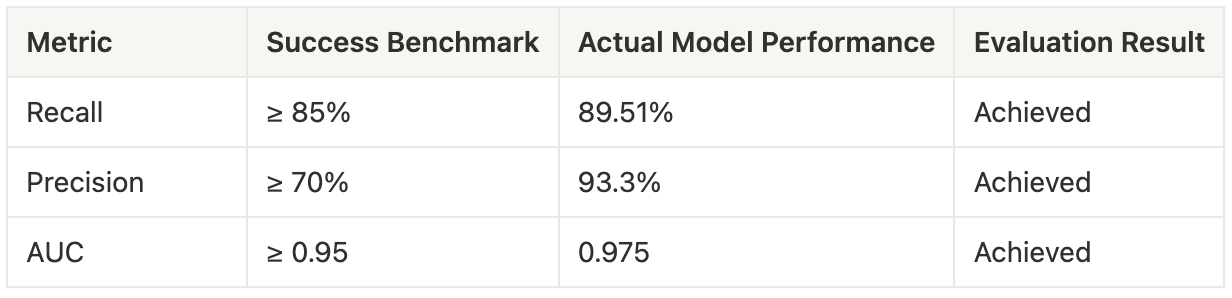
\includegraphics[width=0.5\textwidth]{table5.jpg}
    \caption*{Evaluation of Model Performance Against Success Benchmarks}
    \label{fig:table5}
\end{figure}

This data mining project was a complete success. Through a series of rigorous data processing steps (especially undersampling) and modelling procedures, the logistic regression model I built fully surpassed the predefined core success criteria. The model not only demonstrated outstanding performance from a statistical perspective but also proved to have very high practical value in simulated business scenarios (high precision and high recall). This confirms that the chosen data mining methods and processes are both appropriate and effective.

\subsection{Iterations}

Data mining is not a linear, one-time process but rather a cyclical and continuously optimized iterative process. The logistic regression model I evaluated in Section 8.4, although already surpassing all preset benchmarks, is essentially just my first baseline model. To ensure the final model's validity and robustness, I documented the phenomena observed in this analysis and planned subsequent iterative optimization steps.

\subsubsection{Limitations and Randomness of the Current Model}

During this modeling process, I observed that due to the random sampling mechanisms of the ``Sample'' node and the ``Partition'' node, each rerun of the data flow produced slight fluctuations in performance metrics (such as accuracy). While such fluctuations are normal, they indicate that the model's performance is influenced by specific dataset partitions. To achieve a more stable and trustworthy performance evaluation, and further enhance the model's capability, I have planned the following iterative workflow.

\subsubsection{Subsequent Iteration Plans and Rationale}

I will repeat steps of data transformation, modeling, and evaluation, focusing on the following three iterative optimizations to ensure the model remains effective and robust:

\textbf{Iteration One: Stabilizing the Baseline}

\begin{itemize}
    \item \textbf{Steps/Process:} I will revisit the ``Sample'' and ``Partition'' nodes in the data flow and configure them with a fixed random seed, e.g., 2024.
    \item \textbf{Rationale:} This step eliminates randomness in sampling and partitioning, ensuring that each run yields exactly the same dataset and evaluation results. This will provide me with a stable and consistent performance baseline, allowing subsequent optimization attempts to be compared fairly and accurately.
\end{itemize}

\textbf{Iteration Two: Data Transformation \& Feature Engineering}

\begin{itemize}
    \item \textbf{Steps/Process:} Building on the stable baseline model, I will introduce feature scaling. Specifically, I will use a ``Derive'' node to apply Min--Max normalization to features such as amount and oldbalanceOrig, scaling them into the [0, 1] range.
    \item \textbf{Rationale:} The current model's numerical features differ vastly in scale (e.g., amount could be in the millions, while type\_category is only 0 or 1). This disparity may cause large-scale features to dominate model training disproportionately. Normalization eliminates this bias, allowing the model to more fairly evaluate the true contribution of each feature, which could further improve accuracy and stability.
\end{itemize}

\textbf{Iteration Three: Algorithm Comparison \& Parameter Tuning}

\begin{itemize}
    \item \textbf{Steps/Process:}
    \begin{enumerate}
        \item \textbf{Algorithm comparison:} I will introduce other classification algorithms in parallel within the data flow, such as Decision Tree (C5.0) and Neural Network nodes, training and evaluating them on the same dataset.
        \item \textbf{Parameter tuning:} I will leverage SPSS Modeler's automated modeling nodes (e.g., ``Auto Classifier'') or manually adjust advanced parameters of the ``Logistic'' node (such as stepwise method and regularization options) to find the optimal parameter set.
    \end{enumerate}
    \item \textbf{Rationale:} Logistic regression is only one of many strong classification algorithms. Different algorithms have distinct logics and application scenarios. By comparing multiple algorithms side by side, I can ensure that the final choice is the most suitable and best-performing model rather than simply the first successful one. Parameter tuning will then allow me to further refine the chosen model, extracting its final performance potential.
\end{itemize}

Through these planned iterations, I will be able to start from a successful baseline model and progressively build a final model that is more accurate, more stable, and more rationally chosen, ensuring that the outcomes of this data mining project are robust and trustworthy.

%% Example table (uncomment to use)
%%\begin{table}
%%  \caption{Your table caption}
%%  \label{tab:example}
%%  \begin{tabular}{lll}
%%    \toprule
%%    Column 1 & Column 2 & Column 3\\
%%    \midrule
%%    Data 1 & Data 2 & Data 3\\
%%    \bottomrule
%%  \end{tabular}
%%\end{table}

%% Example math equations (uncomment to use)
%%\section{Mathematical Content}
%%Inline math: $\alpha + \beta = \gamma$
%%
%%Display equation:
%%\begin{equation}
%%  \sum_{i=0}^{n} x_i = \int_{0}^{\infty} f(x) dx
%%\end{equation}

%% Example figure (uncomment to use)
%%\begin{figure}[h]
%%  \centering
%%  \includegraphics[width=\linewidth]{your-image}
%%  \caption{Your figure caption.}
%%  \Description{Description of your figure.}
%%  \label{fig:example}
%%\end{figure}

%% Academic Integrity Declaration
\section*{Academic Integrity Declaration}

I acknowledge that the submitted work is my own original work in accordance with the University of Auckland guidelines and policies on academic integrity and copyright. (See: \href{https://www.auckland.ac.nz/en/students/forms-policies-and-guidelines/student-policies-and-guidelines/academic-integrity-copyright.html}{Academic Integrity and Copyright}).

I also acknowledge that I have appropriate permission to use the data that I have utilised in this project. (For example, if the data belongs to an organisation and the data has not been published in the public domain, then the data must be approved by the rights holder.) This includes permission to upload the data file to Canvas. The University of Auckland bears no responsibility for the student's misuse of data.

%% Acknowledgments (optional)
%%\begin{acks}
%%Thank you to...
%%\end{acks}

%% Bibliography
\bibliographystyle{ACM-Reference-Format}
\bibliography{references}  %% Change 'references' to your .bib file name

%% Appendix (optional)
%%\appendix
%%\section{Additional Material}
%%Additional content here...

\end{document}
\endinput
%%
%% End of file `sample-sigplan.tex'.
